% !TeX root = _main.tex
% FILE DIEU PHOI 1/2: preamble, trang bia, muc luc, cau hinh build.
% Chi nguoi ghep bai sua file nay. Noi dung: role_1.tex, role_2.tex, role_3.tex.
\documentclass[12pt,a4paper]{article}
\usepackage{iftex}
\ifPDFTeX
  \usepackage[utf8]{inputenc}
  \usepackage[utf8]{vietnam}
  \usepackage{mathptmx}
\else
  \usepackage{fontspec}
  \setmainfont{texgyretermes}[Extension=.otf,UprightFont=*-regular,
    BoldFont=*-bold,ItalicFont=*-italic,BoldItalicFont=*-bolditalic]
  \setsansfont{texgyreheros}[Extension=.otf,UprightFont=*-regular,
    BoldFont=*-bold,ItalicFont=*-italic,BoldItalicFont=*-bolditalic]
  \setmonofont{lmmono10-regular.otf}[ItalicFont=lmmono10-italic.otf]
\fi
\usepackage[left=30mm,right=20mm,top=20mm,bottom=20mm]{geometry}
\usepackage{amsmath,amssymb}
\usepackage{graphicx,booktabs,tabularx,array,longtable}
\usepackage[table]{xcolor}
\usepackage{setspace,indentfirst,enumitem}
\usepackage{float,placeins,rotating}
\usepackage{tikz}
\usetikzlibrary{calc,positioning,arrows.meta,shapes.geometric,fit,backgrounds}
\usepackage[font=small,labelfont=bf,justification=centering]{caption}
\usepackage[numbers,sort&compress]{natbib}
\usepackage[hidelinks,unicode]{hyperref}
\usepackage{xurl}
\definecolor{lightgray}{gray}{0.95} % Định nghĩa màu xám nhẹ (0.95 gần trắng)
% \usepackage[backend=biber,style=numeric-comp,sorting=none]{biblatex}
% \addbibresource{references.bib}

\setstretch{1.3}
\setlength{\emergencystretch}{2em}
\setlist{nosep,leftmargin=*}
\renewcommand{\arraystretch}{1.18}
\renewcommand{\contentsname}{Mục lục}
\renewcommand{\figurename}{Hình}
\renewcommand{\tablename}{Bảng}
\renewcommand{\refname}{Tài liệu tham khảo}
\renewcommand{\appendixname}{Phụ lục}
\newcolumntype{Y}{X} % can deu hai ben; can trai thi dung >{\raggedright\arraybackslash}X
\hypersetup{pdftitle={Giảm hàng chờ giờ cao điểm tại cửa hàng xăng dầu nội thành Hà Nội},pdfauthor={Nhóm 8 -- INT3501}}

% De hien TODO trong ban lam viec; doi thanh \draftfalse khi cac TODO da xu ly.
% Tat hien thi KHONG thay the viec hoan thanh cong viec.
\newif\ifdraft
\drafttrue
\newcommand{\todo}[2]{\ifdraft\par\smallskip\noindent
  \begingroup\color{red!65!black}\textbf{[TODO -- Role #1]} #2\par\endgroup\smallskip\fi}
\newcommand{\source}[1]{\par\smallskip{\footnotesize\textit{Nguồn: #1.}\par}}
\newcommand{\placeholder}[2]{\begin{center}\fbox{\parbox{0.91\linewidth}{%
  \textbf{Cần bổ sung: #1}\par #2}}\end{center}}
% Bang da sinh tu analysis/ (luu o tables/): giu so lieu goc, tu dong vua kho giay.
\newcommand{\resulttable}[3]{\begin{table}[htbp]\centering
  \caption{#2}\label{#3}
  \resizebox{\linewidth}{!}{\input{tables/#1}}
  % \source{\texttt{tables/\detokenize{#1}}; dữ liệu mô phỏng có sẵn trong dự án}
  \end{table}}
% Bang sinh tu Python giu kich thuoc tu nhien, chi thu nho khi rong hon le.
\newcommand{\exttable}[3]{\begin{table}[htbp]\centering\small
  \caption{#2}\label{#3}
  \resizebox{\ifdim\width>\linewidth\linewidth\else\width\fi}{!}{\input{tables/#1}}
  % \source{\texttt{tables/\detokenize{#1}}; dữ liệu mô phỏng, quy mô hiệu chỉnh từ số liệu công bố}
  \end{table}}
% Ky phap so do quy trinh (BPMN rut gon) dung chung cho role 1 va role 3.
\tikzset{
  task/.style={rectangle,rounded corners=3pt,draw,thick,align=center,font=\scriptsize,
    minimum width=21mm,minimum height=9mm,fill=white},
  gw/.style={diamond,draw,thick,aspect=1.4,align=center,font=\scriptsize,inner sep=1pt,fill=white},
  ev/.style={circle,draw,thick,minimum size=6mm,fill=white},
  evend/.style={circle,draw,line width=2pt,minimum size=6mm,fill=white},
  flow/.style={-{Stealth[length=2mm]},thick},
  msg/.style={-{Stealth[length=2mm,open]},dashed},
  lane/.style={draw,thin,minimum height=17mm,anchor=north west},
  tmark/.style={font=\scriptsize\itshape,text=red!60!black}}

\begin{document}
\hypersetup{pageanchor=false}
\begin{titlepage}

\begin{tikzpicture}[remember picture,overlay]
  \draw[line width=1.5pt] ($(current page.north west)+(25mm,-25mm)$)
    rectangle ($(current page.south east)+(-12mm,25mm)$);
\end{tikzpicture}
\begin{center}
\textbf{ĐẠI HỌC QUỐC GIA HÀ NỘI}\\
\textbf{TRƯỜNG ĐẠI HỌC CÔNG NGHỆ}\\
\textbf{KHOA CÔNG NGHỆ THÔNG TIN}
\vspace{14mm}


\includegraphics[width=0.25\linewidth]{figures/uet.png}
\vspace{12mm}

{\large\bfseries BÁO CÁO CUỐI KỲ}\\[6mm]
{\Large\bfseries KHOA HỌC DỊCH VỤ}\\[8mm]
% \fontsize{20}{24}\selectfont
{\large\bfseries GIẢM HÀNG CHỜ GIỜ CAO ĐIỂM\\TẠI CỬA HÀNG XĂNG DẦU NỘI THÀNH HÀ NỘI}
% Phân tích hàng đợi và đề xuất cải tiến phục vụ\\
% tại cửa hàng xăng dầu nội thành Hà Nội
% }
\end{center}
\vspace{10mm}
\noindent\begin{tabular}{@{}lll@{}}
Mã học phần: & INT3501 1 & \\
Nhóm: & 8 & \\
Sinh viên thực hiện: & Phạm Tuấn Anh & MSSV: 23020010 \\
 & Đoàn Văn Tuyền & MSSV: 23020151 \\
 & Phạm Nam Khánh & MSSV: 23020088 \\
Giảng viên môn học: & \multicolumn{2}{l}{TS. Nguyễn Thị Cẩm Vân} \\
\end{tabular}
\vfill
\begin{center}\textbf{HÀ NỘI -- 2026}\end{center}
\vspace*{12mm}
\end{titlepage}
\pagenumbering{roman}
\hypersetup{pageanchor=true}
\tableofcontents
\clearpage

\pagenumbering{arabic}

% !TeX root = _main.tex
% FILE DIEU PHOI 2/2: thu tu ghep, tai lieu tham khao, phu luc chung.
% Nguoi ghep bai quan ly file nay. KHONG viet lai noi dung cua cac role o day.
% Role 1 (Tuan Anh): muc 1--4; Role 2 (Tuyen): muc 5--7 va Phu luc B;
% Role 3 (Khanh): muc 8--10.
% !TeX root = _main.tex
% ROLE 1: muc 1--4, van de, pham vi, he thong, nguon luc va AS-IS.
% Chi sua role cua minh va figures/rX_*. Khong sua tay bang do Python sinh.
% Nguoi ghep bai quan ly _main.tex va _content.tex.
% Macro Role*Supplement cuoi file giu ban nhap mo rong; KHONG duoc goi trong PDF.

\section{Bài toán, mục tiêu và phạm vi nghiên cứu}
\label{r1:scope}
\subsection{Bối cảnh và vấn đề cần giải quyết}
Hà Nội có 453 cửa hàng bán lẻ xăng dầu và nhu cầu tiêu thụ khoảng
110\,000~m$^3$ xăng/tháng theo số liệu được công bố tháng 3/2026~\cite{sct2026}.
Các số liệu này cung cấp quy mô tham chiếu, không mô tả lượng khách của một
cửa hàng cụ thể. Nhóm xét một cửa hàng giả định có 8 vòi bơm, phục vụ trong
khung 06:00--22:00, với lượng xe thay đổi theo giờ.

\textbf{Vấn đề dịch vụ.} Khách có thể phải chờ lâu hoặc bỏ đi vào giờ cao
điểm, trong khi một số giờ khác còn dư công suất. Báo cáo cần trả lời liệu
việc giữ số nhân viên cố định và thời gian chiếm trụ có góp phần tạo hàng
chờ hay không. Đây là giả thuyết được kiểm tra bằng mô phỏng; chưa phải
kết luận về một cửa hàng đã khảo sát.

\textbf{Ảnh hưởng.} Khách mất thời gian và có thể không mua được xăng;
nhân viên chịu áp lực không đều trong ngày; cửa hàng phải cân đối mức phục
vụ với chi phí nhân lực. Vì vậy, chỉ nhìn thời gian chờ trung bình cả ngày
hoặc tăng nhân viên cho mọi giờ đều chưa đủ căn cứ.

\subsection{Câu hỏi phân tích và mạch lập luận}
\textbf{Câu hỏi chính.} Có thể giảm tỷ lệ chờ quá 5 phút và tỷ lệ bỏ đi ở
khung 17:00--19:00 bằng cách điều chỉnh số kênh phục vụ theo giờ hay không,
và khi nào nên thử thêm cải tiến thanh toán?
\begin{table}[H]\centering\small
\caption{Mạch phân tích của báo cáo}\label{r1:problems}
\begin{tabularx}{\linewidth}{@{}p{28mm}Y Y@{}}
\toprule
Bước & Câu hỏi cần trả lời & Bằng chứng / đầu ra \\
\midrule
Nêu vấn đề & Chờ ở đâu, lúc nào, ảnh hưởng ai? & AS-IS, mốc đo, chỉ số theo giờ và tỷ lệ bỏ đi. \\
Phân tích nguyên nhân & Nhu cầu có vượt công suất? Trụ bị chiếm bởi thao tác nào? & $\lambda_t$, $c_t$, thời gian phục vụ; so sánh giả thuyết với mô hình. \\
Đề xuất giải pháp & Thay đổi gì để tác động đúng nguyên nhân? & A1 điều chỉnh công suất theo giờ; A2 thử giảm thời gian thanh toán tại trụ. \\
Đánh giá & Khách chờ ít hơn không? Chi phí và điều kiện thực hiện là gì? & Cùng dòng xe cho A0/A1/A2; độ nhạy, rủi ro và kế hoạch thử nghiệm. \\
\bottomrule
\end{tabularx}
\end{table}
Bài toán chính là hàng đợi và phân bổ công suất. Định vị cửa hàng, học máy
và chiến lược dài hạn được giữ ở bản nháp mở rộng, chưa dùng làm căn cứ cho
khuyến nghị của báo cáo này.

\subsection{Ranh giới hệ thống và ranh giới phép đo}
\begin{table}[htbp]\centering\small
\caption{Phạm vi dịch vụ và phạm vi mô hình định lượng}\label{r1:boundary}
\begin{tabularx}{\linewidth}{@{}p{32mm}Y@{}}
\toprule
Thành phần & Mô tả \\
\midrule
Khách hàng & Hai loại xe theo giả định: xe máy (97,3\% lượt) và ô tô (2,7\% lượt). \\
Tác nhân cung cấp & Nhân viên bơm, cửa hàng trưởng, doanh nghiệp đầu mối, ngân hàng/ví điện tử, cơ quan thuế. \\
Trigger dịch vụ & Xe vào cửa hàng và nhìn thấy hàng chờ tại các trụ bơm. \\
Outcome dịch vụ & Xe được bơm đủ, thanh toán xong, có hóa đơn điện tử và rời trụ. \\
Đầu vào mô hình & Thời điểm xe vào hàng chờ $a_i$ (hoặc bỏ đi nếu hàng quá dài). \\
Đầu ra mô hình & Thời điểm rời trụ $d_i$; $W_q=b_i-a_i$ với $b_i$ là lúc nhân viên bắt đầu phục vụ. \\
Ngoài mô hình & Chất lượng xăng, nhập hàng và tồn kho bể, an toàn phòng cháy, dịch vụ phụ (rửa xe, cửa hàng tiện lợi). \\
\bottomrule
\end{tabularx}
\end{table}
Cửa hàng có thể mở 24 giờ, nhưng phân tích chỉ xét 06:00--22:00, nơi tập
sinh toàn bộ lượt xe của kịch bản; nhu cầu ngoài giờ chưa được xét. Mỗi ``kênh'' trong mô hình là một vòi bơm có
nhân viên phục vụ; số kênh không vượt quá 8 vòi vật lý.

\subsection{Mục tiêu và tiêu chí đánh giá}
Mục tiêu là cải thiện khả năng phục vụ giờ cao điểm với chi phí nhân lực
hợp lý. Nhóm đề xuất các ngưỡng để so sánh phương án: thời gian chờ trung
bình không quá 2 phút, tỷ lệ chờ quá 5 phút không quá 5\%, tỷ lệ bỏ đi không
quá 1\%. Đây là mục tiêu nghiên cứu, cần thống nhất lại với cửa hàng nếu
triển khai. Báo cáo đánh giá riêng cả ngày và khung 17:00--19:00, đồng thời
so sánh giờ công, chi phí và mức chịu tải khi nhu cầu tăng.

Không đặt trước một tỷ lệ cắt giảm nhân lực phải đạt: phương án chỉ được
đề xuất nếu giữ chất lượng phục vụ và có thể chuyển thành lịch ca thực tế.

\section{Mô hình hệ thống dịch vụ}
\label{r1:system}
Báo cáo dùng mô hình hệ thống dịch vụ làm khung chủ đạo để liên kết tác nhân,
nguồn lực, hoạt động, thông tin, quy tắc và kết quả~\cite{rubric}.
\begin{table}[htbp]\centering\small
\caption{Các thành phần của hệ thống và liên hệ với bài toán chờ}\label{r1:components}
\begin{tabularx}{\linewidth}{@{}p{24mm}Y Y@{}}
\toprule
Thành phần & Biểu hiện tại cửa hàng & Liên hệ với phân tích \\
\midrule
Con người & Khách xe máy/ô tô, nhân viên bơm, cửa hàng trưởng & Số kênh có nhân viên $c_t$; tỷ trọng loại xe. \\
Hoạt động & Mời xe vào trụ, bơm, thu tiền, xuất hóa đơn & Thời gian phục vụ $S$ theo loại xe. \\
Thông tin & Giá niêm yết, số tiền/số lít, hóa đơn điện tử & Dữ liệu từng lần bán dùng để dự báo $\lambda_t$. \\
Công nghệ & Cột bơm, máy POS, QR/ví, ứng dụng trả trước & Số hóa giảm thời gian thanh toán (A2). \\
Quy tắc & FCFS tại mỗi trụ, hóa đơn từng lần bán, giờ mở cửa & Ràng buộc $c_t\le8$; mục tiêu thời gian chờ. \\
Kết quả & Xe được phục vụ, khách quay lại & $W_q$, $P(W_q{>}5)$, tỷ lệ bỏ đi, chi phí. \\
\bottomrule
\end{tabularx}
\end{table}

\section{Bản đồ nguồn lực và cơ chế đồng tạo giá trị}
\label{r1:resources}
\begin{figure}[htbp]\centering
\resizebox{0.95\linewidth}{!}{%
\begin{tikzpicture}[node distance=10mm,
  hub/.style={rectangle,rounded corners=4pt,draw,very thick,fill=blue!6,align=center,font=\small,minimum width=34mm,minimum height=12mm},
  act/.style={rectangle,rounded corners=3pt,draw,thick,fill=gray!8,align=center,font=\scriptsize,minimum width=27mm,minimum height=9mm},
  res/.style={font=\scriptsize\itshape,align=center,fill=white,inner sep=1pt}]
\node[hub] (s) at (0,0) {Cửa hàng xăng dầu\\(8 vòi, nhân viên bơm)};
\node[act] (c) at (-6.2,2.4) {Khách xe máy / ô tô\\(theo thế hệ)};
\node[act] (b) at (6.2,2.4) {Doanh nghiệp đầu mối\\(nguồn hàng, chiết khấu)};
\node[act] (p) at (-6.2,-2.4) {Ngân hàng / ví điện tử\\(QR, trả trước)};
\node[act] (t) at (6.2,-2.4) {Cơ quan thuế,\\Sở Công Thương};
\node[act] (e) at (0,-3.6) {Đối tác trạm sạc / đổi pin};
\draw[<->,thick] (c) -- node[res]{tiền, thời gian,\\dữ liệu mua hàng} (s);
\draw[<->,thick] (b) -- node[res]{xăng, giá bán lẻ\\$\leftrightarrow$ sản lượng} (s);
\draw[<->,thick] (p) -- node[res]{hạ tầng thanh toán\\$\leftrightarrow$ phí giao dịch} (s);
\draw[<->,thick] (t) -- node[res]{quy định, hóa đơn\\từng lần bán} (s);
\draw[<->,thick,dashed] (e) -- node[res]{mặt bằng $\leftrightarrow$ khách xe điện} (s);
\end{tikzpicture}}
\caption{Bản đồ nguồn lực của cửa hàng xăng (nét đứt: quan hệ tương lai khi chuyển dịch xe điện).}
\label{r1:resource-map}
\source{nhóm vẽ bằng TikZ dựa trên các tác nhân trong Bảng~\ref{r1:components}; Claude Code hỗ trợ dựng mã hình}
\end{figure}
Khách hàng góp thời gian chờ, tiền và dữ liệu mua hàng; nhân viên góp thao tác
phục vụ; đầu mối cung cấp nguồn hàng và chiết khấu; ngân hàng/ví cung cấp
thanh toán số; cơ quan thuế đặt quy tắc hóa đơn. Giá trị (``vào là được bơm
ngay'') chỉ xuất hiện khi các nguồn lực này khớp với nhau theo giờ: thiếu nhân
viên giờ tan tầm hoặc thao tác thanh toán chậm đều chuyển chi phí sang thời
gian chờ của khách. Hai cơ chế này tương ứng với hai biến quyết định $c_t$ và
$E[S]$ của mô hình.

\begin{table}[htbp]\centering\small
\caption{Lợi ích các bên và điều kiện chấp nhận giải pháp}\label{r1:stakeholders}
\begin{tabularx}{\linewidth}{@{}p{25mm}Y Y Y@{}}
\toprule
Bên liên quan & Lợi ích hiện tại & Kỳ vọng dự kiến & Điều kiện cải tiến \\
\midrule
Khách dùng QR & Thanh toán thuận tiện & Chờ ít hơn, giao dịch chính xác & Đo thời gian và lỗi giao dịch khi thử A2 \\
Khách dùng tiền mặt & Nhân viên hỗ trợ, trả tiền mặt & Vẫn được phục vụ khi không dùng ứng dụng & Giữ kênh tiền mặt, không ép số hóa \\
Nhân viên bơm & Lương 8--12 triệu đồng/tháng~\cite{wage} & Ca ổn định, không quá tải giờ cao điểm & Lịch theo giờ cần báo trước, có ca linh hoạt có thù lao \\
Đầu mối cung ứng & Sản lượng ổn định & Cung ứng đúng kế hoạch & Phân biệt thiếu hàng với thiếu công suất phục vụ \\
Cơ quan quản lý & Giao dịch minh bạch & Thông tin đầy đủ, có thể đối soát & Không bỏ bước kiểm tra để rút ngắn thời gian \\
\bottomrule
\end{tabularx}
\end{table}

\section{Quy trình hiện tại và chẩn đoán điểm nghẽn}
\label{r1:asis}
\subsection{Hành trình khách hàng và blueprint AS-IS}
Hành trình gồm: thấy cửa hàng $\rightarrow$ quyết định vào hay đi tiếp (nhìn độ
dài hàng) $\rightarrow$ chờ $\rightarrow$ mở nắp bình, báo số tiền $\rightarrow$
bơm $\rightarrow$ thanh toán, nhận hóa đơn $\rightarrow$ rời trụ.
Hai điểm đau chính là \emph{không đoán được phải chờ bao lâu} khi nhìn hàng
và \emph{thao tác thanh toán bằng tiền mặt, trả lại tiền thừa, xuất hóa đơn}
kéo dài thời gian chiếm trụ.
\begin{table}[htbp]\centering\small
\caption{Các lớp của blueprint tại điểm chờ}\label{r1:blueprint}
\begin{tabularx}{\linewidth}{@{}p{34mm}Y@{}}
\toprule
Lớp & Nội dung \\
\midrule
Bằng chứng hữu hình & Biển giá, đồng hồ cột bơm, hàng xe đang chờ, hóa đơn điện tử. \\
Hành động khách & Chọn trụ, xếp hàng, mở nắp bình, báo số tiền, thanh toán. \\
\multicolumn{2}{@{}c@{}}{\footnotesize\textit{--- đường tương tác ---}} \\
Tuyến trước & Nhân viên mời xe, bơm, thu tiền, trả tiền thừa. \\
\multicolumn{2}{@{}c@{}}{\footnotesize\textit{--- đường nhìn thấy ---}} \\
Tuyến sau & Máy POS ghi giao dịch, xuất hóa đơn điện tử từng lần bán. \\
Quy trình hỗ trợ & Lịch ca, nhập hàng, đối soát tiền mặt cuối ca, kết nối cơ quan thuế. \\
\bottomrule
\end{tabularx}
\end{table}

\subsection{Sơ đồ quy trình AS-IS (BPMN rút gọn)}
\begin{figure}[htbp]\centering
\resizebox{\linewidth}{!}{%
\begin{tikzpicture}
\def\W{18.4}
\foreach \y/\name in {0/Khách hàng,-2.4/Nhân viên bơm,-4.8/Hệ thống POS / HĐĐT}{
  \draw (0,\y) rectangle (\W,\y-2.4);
  \draw (0.8,\y) -- (0.8,\y-2.4);
  \node[rotate=90,font=\scriptsize\bfseries] at (0.4,\y-1.2) {\name};}
\node[ev] (st) at (1.6,-1.2) {};
\node[task] (t1) at (3.4,-1.2) {Xe vào\\cửa hàng};
\node[gw] (g1) at (5.6,-1.2) {Hàng chờ\\$\ge$ 20 xe?};
\node[evend] (eb) at (7.3,-0.45) {};
\node[font=\scriptsize,anchor=west] at (7.7,-0.45) {bỏ đi (balk)};
\node[task] (t2) at (8.4,-1.6) {Xếp hàng\\chờ tới lượt};
\node[task] (t3) at (10.6,-3.6) {Mời xe vào trụ,\\hỏi số tiền/số lít};
\node[task] (t4) at (13.0,-3.6) {Bơm xăng};
\node[task] (t5) at (13.0,-1.2) {Thanh toán\\tiền mặt / QR};
\node[task] (t6) at (15.6,-6.0) {Xuất hóa đơn\\điện tử từng lần};
\node[task] (t7) at (15.6,-1.2) {Nhận hóa đơn,\\rời trụ};
\node[evend] (en) at (17.7,-1.2) {};
\draw[flow] (st) -- (t1);
\draw[flow] (t1) -- (g1);
\draw[flow] (g1.north) |- node[pos=0.25,left,font=\scriptsize]{có} (eb);
\draw[flow] (g1.east) -- node[above,font=\scriptsize]{không} ++(0.6,0) |- (t2);
\draw[flow] (t2) |- (t3);
\draw[flow] (t3) -- (t4);
\draw[flow] (t4) -- (t5);
\draw[flow] (t5.east) -- ++(0.35,0) |- (t6.west);
\draw[flow] (t6.north) -- (t7.south);
\draw[flow] (t7) -- (en);
\node[tmark,anchor=west] at (9.5,-1.6) {$a_i$: vào hàng};
\node[tmark] at (10.6,-4.35) {$b_i$: bắt đầu phục vụ};
\node[tmark] at (15.6,-0.35) {$d_i$: rời trụ};
\end{tikzpicture}}
\caption{Quy trình AS-IS tại một vòi bơm; nhãn đỏ là các mốc thời gian dùng để đo $W_q=b_i-a_i$ và $S=d_i-b_i$.}
\label{r1:bpmn}
\source{nhóm vẽ bằng TikZ theo ký pháp BPMN rút gọn (sự kiện, tác vụ, cổng XOR, làn); Claude Code hỗ trợ dựng mã hình}
\end{figure}
Thời gian phục vụ $S$ gồm cả bơm, thanh toán và xuất hóa đơn: trụ chỉ được giải
phóng khi khách rời đi. Nếu giảm được thao tác tại trụ, A2 có thể rút ngắn
thời gian chiếm trụ dù tốc độ bơm không đổi.
\todo{1}{Đối chiếu sơ đồ với quan sát tại một cửa hàng thật (bấm giờ 30--50 lượt
mỗi loại xe), sửa nhánh ngoại lệ nếu có (hết loại xăng, lỗi POS).}

\subsection{Từ điểm nghẽn đến biến đo}
\begin{table}[htbp]\centering\small
\caption{Giả thuyết chẩn đoán và biến kiểm tra}\label{r1:diagnosis}
\begin{tabularx}{\linewidth}{@{}Y Y Y@{}}
\toprule
Điểm trên quy trình & Cơ chế giả định & Biến kiểm tra \\
\midrule
Hàng dài giờ tan tầm & Lịch nhân viên cố định trong khi lượt xe dao động theo giờ & $\lambda_t$, $c_t$, $\rho_t$, $W_q$ theo giờ \\
Khách bỏ đi & Thấy hàng dài nên sang cửa hàng khác & Tỷ lệ bỏ đi (balking) \\
Chiếm trụ lâu & Tiền mặt, tiền thừa, hóa đơn từng lần bán & $E[S]$ theo loại xe; CV \\
Ngày có sự kiện & Lượng xe tăng ngoài cấu hình cơ sở & $\lambda_t$, hàng chờ và tỷ lệ bỏ đi \\
\bottomrule
\end{tabularx}
\end{table}


% Ban nhap bo tro: chua dua vao PDF chinh.
\newcommand{\RoleOneSupplement}{%
\subsection{Môi trường chiến lược: SWOT và PESTEL}
\begin{table}[htbp]\centering\small
\caption{SWOT của cửa hàng đại diện}\label{r1:swot}
\begin{tabularx}{\linewidth}{@{}Y Y@{}}
\toprule
\textbf{Điểm mạnh (S)} & \textbf{Điểm yếu (W)} \\
Vị trí nội thành, lượng khách lớn; có dữ liệu hóa đơn từng lần bán để đo và dự báo nhu cầu. &
Lịch nhân viên cố định; thanh toán tiền mặt kéo dài thời gian chiếm trụ; tối đa 8 vòi. \\
\midrule
\textbf{Cơ hội (O)} & \textbf{Thách thức (T)} \\
Thanh toán QR/ứng dụng trả trước; dùng mặt bằng cho trạm sạc, đổi pin~\cite{vgx}; đối thủ đóng cửa khi chiết khấu thấp. &
Chuyển dịch sang xe điện và vùng phát thải thấp~\cite{ct20,lez2026}; đứt gãy nguồn cung~\cite{vtc2026}; biên lợi nhuận mỏng~\cite{chietkhau}. \\
\bottomrule
\end{tabularx}
\end{table}

\begin{table}[htbp]\centering\small
\caption{PESTEL: yếu tố dẫn dắt và kịch bản tương ứng ở Mục~\ref{r3:scenarios}}\label{r1:pestel}
\begin{tabularx}{\linewidth}{@{}p{21mm}Y p{17mm}@{}}
\toprule
Yếu tố & Biểu hiện có nguồn & Kịch bản \\
\midrule
Chính trị (P) & Chỉ thị 20/CT-TTg; Đề án vùng phát thải thấp trong Vành đai~1 từ 1/7/2026, cấm theo khung giờ tại khu vực thí điểm~\cite{ct20,lez2026} & KB-A \\
Kinh tế (E) & Giá điều chỉnh hằng tuần (kỳ 5/11/2026 giảm 2\,075 đồng/lít, kỳ 12/11 giảm 1\,310 đồng/lít~\cite{moit2026}); chiết khấu bán lẻ thấp~\cite{chietkhau} & KB-B, KB-C \\
Xã hội (S) & Hà Nội đăng ký mới hơn 255\,000 xe máy năm 2025~\cite{reg2025}; xe máy xăng vẫn chiếm 97\% trong Vành đai~1~\cite{xe97} & KB-B \\
Công nghệ (T) & Thanh toán QR, hóa đơn điện tử; mạng lưới đổi pin tại cửa hàng xăng~\cite{vgx} & KB-A \\
Môi trường (E) & Mục tiêu giảm phát thải giao thông đô thị & KB-A \\
Pháp lý (L) & Hóa đơn điện tử từng lần bán (NĐ 70/2025)~\cite{nd70}; lộ trình cấm có thể lùi tới 2028~\cite{tt2028} & Mọi KB \\
\bottomrule
\end{tabularx}
\end{table}
Các yếu tố trên cho thấy hai bất định lớn: \emph{chiều nhu cầu} (giảm do xe
điện hay tăng do đối thủ đóng cửa) và \emph{cú sốc ngắn hạn} (đứt gãy nguồn
cung, điều chỉnh giá). Đây là cơ sở để xây ba kịch bản A/B/C ở Mục~\ref{r3:scenarios}.
\todo{1}{Mở và đọc lại từng nguồn báo chí/văn bản trong \texttt{thebibliography}
trước khi nộp; nếu nội dung khác số liệu trích, báo người ghép bài sửa.}

}

\FloatBarrier
% \clearpage
% !TeX root = _main.tex
% ROLE 2: muc 5--6, du lieu, phuong phap, phan tich va nguyen nhan.
% Chi sua role cua minh va figures/rX_*. Khong sua tay bang do Python sinh.
% Nguoi ghep bai quan ly _main.tex va _content.tex.
% Cong thuc, bang so chi tiet va bieu mau o role_2_appendix.tex (Phu luc B).
% Macro Role*Supplement cuoi file giu ban nhap mo rong; KHONG duoc goi trong PDF.

\section{Dữ liệu, giả định và phương pháp phân tích}
\label{r2:method}
\subsection{Dữ liệu và giả định}
Nhóm chưa có dữ liệu giao dịch của một cửa hàng thật, nên lượt xe đến trong
báo cáo là \textbf{dữ liệu mô phỏng}. Tuy vậy, quy mô cửa hàng được ước tính từ
số liệu công bố chứ không đặt tùy ý. Hà Nội bán khoảng 110\,000~m$^3$ xăng mỗi
tháng qua 453 cửa hàng~\cite{sct2026}, tức trung bình khoảng 8\,100 lít mỗi
cửa hàng mỗi ngày. Chia lượng xăng này theo số lít mỗi lần đổ, một cửa hàng
đại diện có khoảng 2\,495 lượt xe mỗi ngày. Cách tính chi tiết nằm ở
Phụ lục~\ref{r2:app-params}. Để kiểm tra cách chia lượt xe theo giờ, nhóm dùng
thêm dữ liệu Google Maps của hai cửa hàng tại Hà Nội (Mục~\ref{r2:gmaps}).

Bảng~\ref{r2:assumptions} liệt kê mọi tham số đầu vào và ghi rõ mỗi tham số
lấy từ đâu. Nhãn E là ước tính suy ra từ số liệu công bố, nhãn G là giả định
của nhóm và cần đo lại. Điều đáng chú ý là chỉ ba tham số có nhãn E, còn chín
tham số còn lại đều là G. Nói cách khác, quy mô cửa hàng có căn cứ, nhưng nhịp
xe đến theo giờ và tốc độ phục vụ vẫn là giả định. Nhịp xe đến theo giờ đã được
đối chiếu với Google Maps, còn tốc độ phục vụ chưa có cách kiểm tra.

\begin{table}[htbp]\centering\small
\caption{Tham số đầu vào (E: ước tính từ số liệu công bố; G: giả định cần đo lại)}\label{r2:assumptions}
\begin{tabularx}{\linewidth}{@{}>{\raggedright\arraybackslash}p{42mm}>{\raggedright\arraybackslash}p{54mm}p{8mm}Y@{}}
\toprule
Tham số & Giá trị & Loại & Cách đo lại \\
\midrule
Lượng xăng bán / cửa hàng & 8\,094 lít/ngày & E & Sản lượng bán của cửa hàng \\
Lượt xe / ngày & 2\,495 (xe máy 97,3\%) & E & Đếm hóa đơn điện tử \\
Lượt xe theo giờ $\lambda_t$ & 112--225 xe/giờ & G & Đã đối chiếu Google Maps; giờ trên hóa đơn \\
$E[S]$ xe máy / ô tô & 1,5 / 4,0 phút & G & Bấm giờ tại trụ \\
Độ dao động của $S$ & CV = 0,8 & G & Bấm giờ tại trụ \\
Số vòi / nhân viên & 8 vòi; 6 người mỗi giờ & G & Hỏi cửa hàng \\
Ngưỡng bỏ đi & 20 xe đang chờ & G & Đếm xe bỏ đi \\
Mức giảm $E[S]$ khi trả trước & 20\% & G & Thử tại cửa hàng \\
Chi phí nhân viên & 58\,000 đồng/giờ & E & Bảng lương thật \\
Lãi gộp bán lẻ & 1\,500 đồng/lít & G & Số liệu cửa hàng \\
Chi phí số hóa & 250\,000 đồng/ngày & G & Báo giá \\
Mục tiêu dịch vụ & $E[W_q]\le2$ phút; $P(W_q{>}5)\le5\%$; bỏ đi $\le1\%$ & G & Nhóm đặt \\
\bottomrule
\end{tabularx}
\source{nhóm tổng hợp; căn cứ và nguồn của từng dòng ở Bảng~\ref{r2:assumptions-detail}, Phụ lục~\ref{r2:app-params}}
\end{table}

Trong các giả định, thời gian phục vụ trung bình $E[S]$ ảnh hưởng mạnh nhất,
vì nó quyết định mỗi nhân viên phục vụ được bao nhiêu xe trong một giờ.
Nghiên cứu duy nhất nhóm tìm được có số đo là một trạm ven quốc lộ ở
Indonesia, với 3,89 phút cho một xe máy~\cite{batui}. Trạm này chỉ có 2 làn xe
máy và khoảng 28 xe mỗi giờ, nên con số trên không dùng được cho cửa hàng nội
thành. Với 8 vòi và 225 xe trong giờ cao điểm, mỗi xe
phải được phục vụ dưới 2,13 phút thì hàng chờ mới không dài ra mãi. Nếu mỗi
xe mất 3,89 phút, cửa hàng cần ít nhất 15 nhân viên bơm cùng lúc, quá xa so
với quy mô thực tế. Vì vậy nhóm chọn 1,5 phút cho xe máy, 4 phút cho ô tô, và
coi đây là giá trị cần bấm giờ lại đầu tiên.

Một quan sát khác là ô tô chiếm ít lượt nhưng giữ trụ lâu. Ô tô chỉ chiếm
2,7\% số lượt, nhưng mỗi xe đứng ở trụ lâu gấp 2,7 lần xe máy, nên chiếm
khoảng 7\% tổng thời gian bơm. Tỷ lệ này nhỏ, nên mô hình cho hai loại xe dùng
chung một hàng chờ, với thời gian phục vụ bình quân 1,57 phút.

\subsection{Phương pháp phân tích}
Nhóm dùng hai công cụ bổ sung cho nhau: công thức hàng đợi M/M/c và mô phỏng.
Các ký hiệu $a_i$, $b_i$, $d_i$, $W_q$, $\lambda_t$, $c_t$ và hệ số tải
$\rho$ giữ nguyên định nghĩa ở Mục~\ref{r1:system}. Ba chỉ số chính là thời
gian chờ trung bình $W_q$, tỷ lệ xe chờ quá 5 phút $P(W_q{>}5)$ và tỷ lệ xe
bỏ đi vì hàng quá dài.

Công thức M/M/c cho phép tính nhanh thời gian chờ của từng giờ khi biết
$\lambda_t$, $c_t$ và $E[S]$. Công thức này giả định xe đến ngẫu nhiên theo
phân phối Poisson, thời gian phục vụ theo phân phối mũ, và hàng chờ đã ở trạng
thái ổn định, tức không còn dài thêm hay ngắn đi theo thời gian. Các công thức
lấy theo bài giảng L4~\cite{l4} và được trình bày ở
Phụ lục~\ref{r2:app-formula}. Nhóm dùng công thức này để tìm những giờ thiếu
nhân viên và chọn số kênh sơ bộ.

Mô phỏng dùng để kiểm tra những điều công thức không mô tả được. Chương trình
sinh từng xe đến theo giờ, gán loại xe và thời gian phục vụ, rồi phục vụ theo
thứ tự xe đến trước được bơm trước. Khác với công thức, mô phỏng có hai loại
xe và cho xe bỏ đi khi đã có 20 xe chờ. Số nhân viên trong mô phỏng cũng được
đổi theo từng giờ. Thời gian phục vụ có hệ số biến thiên CV (độ lệch chuẩn
chia cho trung bình) bằng 0,8, tức ít dao động hơn phân phối mũ (CV = 1). Mỗi
phương án được chạy 20 ngày; mã nguồn và nhật ký chạy nằm trong thư mục
\texttt{analysis/}~\cite{analysis}.

\section{Kiểm chứng và phân tích hiện trạng}
\label{r2:diagnosis}
\subsection{Nhu cầu theo giờ}
Hình~\ref{r2:arrivals} cho thấy lượt xe dồn vào buổi chiều tối rõ hơn nhiều so
với buổi sáng. Theo giả định G, cửa hàng có hai đỉnh lúc đi làm và tan tầm.
Giờ đông nhất là 18--19 giờ với 225 xe, gấp đôi giờ vắng nhất. Ba giờ cao
điểm 08--09, 17--18 và 18--19 chỉ chiếm 3/16 thời gian mở cửa nhưng nhận tới
26\% tổng số lượt xe.

\begin{figure}[htbp]\centering
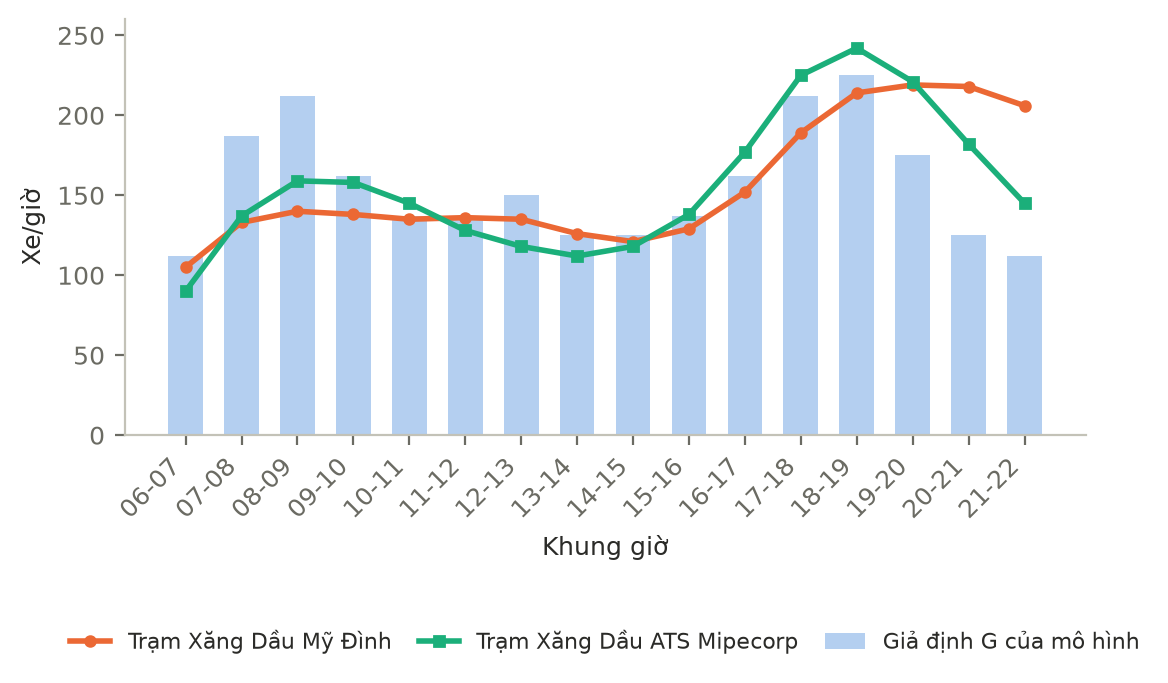
\includegraphics[width=0.78\linewidth]{figures/r2_gmaps.png}
\caption{Lượt xe theo giờ: giả định G của mô hình và phân bố suy từ Google Maps của hai trạm (cùng tổng 2\,495 lượt/ngày)}\label{r2:arrivals}
\source{\texttt{analysis/run\_analysis.py}, \texttt{analysis/gmaps.py}; ảnh Google Maps~\cite{gmaps2026}; số liệu ở Bảng~\ref{r2:gmaps-share}, Phụ lục~\ref{r2:app-tables}}
\end{figure}

Để kiểm tra giả định này, nhóm dùng biểu đồ ``Giờ đông khách'' của Google
Maps. Biểu đồ cho biết mỗi giờ một địa điểm đông đến mức nào so với giờ đông
nhất trong tuần của chính địa điểm đó. Google tính mức này từ vị trí ẩn danh
của người dùng điện thoại, lấy trung bình trong vài tháng gần
nhất~\cite{gmapshelp}. Nhóm chụp biểu đồ đủ 7 ngày của Trạm Xăng Dầu Mỹ Đình
(Lê Quang Đạo) và Trạm Xăng Dầu ATS Mipecorp (Phạm Hùng), đo chiều cao từng cột rồi đổi thành tỷ trọng
theo giờ~\cite{gmaps2026}. Biểu đồ không cho số xe, nên tổng lượt mỗi ngày vẫn
giữ 2\,495. Cách đo nằm ở Phụ lục~\ref{r2:app-plan}.

Dữ liệu của hai trạm chỉ xác nhận đỉnh buổi chiều. Buổi sáng không có đỉnh rõ:
giờ 07--09 chỉ có 133--159 xe, thấp hơn giả định 187--212 xe. Ngược lại, đỉnh
chiều đến muộn hơn và kéo dài hơn. Trạm Mỹ Đình giữ mức 214--219 xe từ 18 đến
21 giờ, và còn 206 xe lúc 21--22 giờ, trong khi giả định chỉ có 112 xe. Trạm
ATS Mipecorp có đỉnh cao hơn giả định, 242 xe lúc 18--19 giờ. Ở cả hai trạm,
giờ đông nhất của hầu hết các ngày là 18--19 giờ. Riêng lúc 20--21 giờ tối thứ
Tư, trạm Mỹ Đình đông gấp 1,5--1,9 lần cùng giờ các ngày khác; nhóm chưa rõ
nguyên nhân.

Sự chênh lệch giữa giờ vắng và giờ đông là gốc của hàng chờ khi lịch nhân viên
cố định. Với 6 nhân viên suốt ngày, công suất cửa hàng không đổi, trong khi
nhu cầu thay đổi khoảng gấp đôi trong ngày. Các phân tích còn lại của báo cáo
vẫn dùng giả định G làm đường cơ sở; phân bố Google Maps được dùng để kiểm tra
lại ở Mục~\ref{r2:gmaps}. Bộ dữ liệu mô phỏng theo giả định G có 50\,144 lượt
xe trong 20 ngày, thời gian phục vụ trung bình 1,568 phút, khớp với tham số đã
đặt (Bảng~\ref{r2:lambda}). Điều này chỉ cho thấy mã chạy đúng thiết kế.

\subsection{Độ tin cậy của công thức M/M/c}
Hình~\ref{r2:validation}a cho thấy công thức và mô phỏng khớp nhau khi tải
vừa phải nhưng lệch xa khi tải gần đầy. Để so sánh công bằng, mô phỏng ở đây
dùng đúng giả định của công thức: một loại xe, thời gian phục vụ phân phối mũ
và không có xe bỏ đi. Với hệ số tải $\rho$ từ 0,73 đến 0,84, hai cách tính
chênh nhau không quá 7,5\%. Ở $\rho=0{,}98$, công thức cho 12,17 phút còn mô
phỏng chỉ cho 7,61 phút, thấp hơn 37,5\%.

\begin{figure}[htbp]\centering
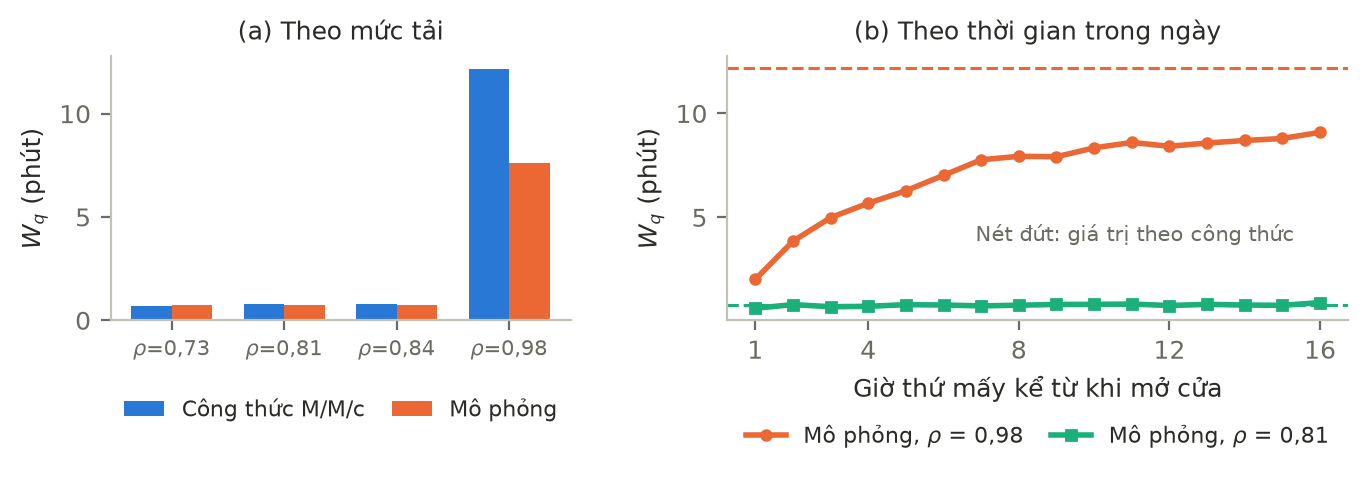
\includegraphics[width=0.86\linewidth]{figures/r2_validation.png}
\caption{So sánh công thức M/M/c với mô phỏng: (a) theo mức tải; (b) thời gian chờ theo giờ kể từ khi mở cửa}\label{r2:validation}
\source{\texttt{analysis/run\_analysis.py}; mô phỏng 40 ngày mỗi cấu hình ở (a), 200 ngày ở (b); số liệu ở Bảng~\ref{r2:validation-table}}
\end{figure}

Chênh lệch này không có nghĩa là mô phỏng sai. Khi tải gần đầy, hàng chờ cần
rất nhiều giờ mới đạt trạng thái ổn định mà công thức giả định. Hình~\ref{r2:validation}b
theo dõi thời gian chờ theo từng giờ kể từ khi mở cửa, khi mỗi ngày bắt đầu
không có xe chờ. Ở $\rho=0{,}81$, thời gian chờ gần bằng giá trị công thức ngay
từ giờ thứ hai. Ở $\rho=0{,}98$, thời gian chờ tăng dần từ 2,0 phút ở giờ đầu
lên 9,1 phút ở giờ thứ 16 mà vẫn chưa chạm mức công thức. Khi nhóm chạy mô
phỏng liên tục 3\,000 giờ, kết quả trung bình của ba lần chạy là 12,32 phút,
rất gần 12,17 phút của công thức. Như vậy, cả hai cách tính đều đúng; chênh
lệch đến từ việc một ngày làm việc quá ngắn để hàng chờ kịp ổn định.

Giờ cao điểm thật chỉ kéo dài một đến hai giờ, nên ở những giờ này công thức
báo thời gian chờ cao hơn thực tế. Vì vậy, nhóm dùng công thức như một phép
kiểm tra thận trọng để tìm giờ thiếu nhân viên, còn mức chờ cụ thể lấy từ mô
phỏng.

\subsection{Điểm nghẽn của lịch hiện tại}
Hình~\ref{r2:asis-load} cho thấy lịch 6 nhân viên cố định thừa người trong
phần lớn thời gian nhưng thiếu người đúng lúc đông nhất. Trong 16 giờ mở cửa,
13 giờ đạt mục tiêu, và từ 09:00 đến 17:00 hệ số tải chỉ từ 0,54 đến 0,71.
Ba giờ còn lại không đạt. Riêng giờ 18--19 có $\rho=0{,}98$, và theo công
thức khoảng 64\% xe phải chờ quá 5 phút.

\begin{figure}[htbp]\centering
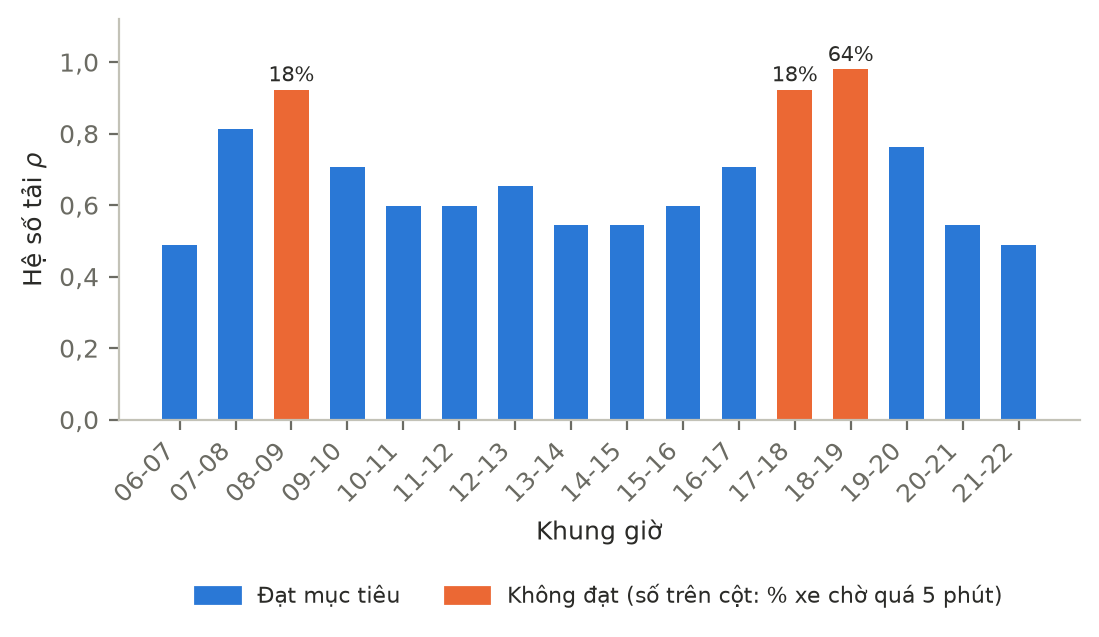
\includegraphics[width=0.7\linewidth]{figures/r2_asis_load.png}
\caption{Hệ số tải theo giờ của lịch hiện tại (6 nhân viên, $E[S]=1{,}57$ phút, công thức M/M/c)}\label{r2:asis-load}
\source{\texttt{analysis/run\_analysis.py}; số liệu đầy đủ ở Bảng~\ref{r2:hourly}, Phụ lục~\ref{r2:app-tables}}
\end{figure}

Vấn đề vì vậy không nằm ở tổng số giờ công mà ở cách chia giờ công trong
ngày. Nếu mỗi giờ chỉ bố trí số nhân viên ít nhất mà vẫn đạt mục tiêu (cách
tính ở Mục~\ref{r3:tobe}), lịch hiện tại thừa 11 giờ công ở các giờ vắng và
thiếu 3 giờ công ở ba giờ cao điểm. Khi $\rho$ vượt khoảng 0,9, gần như không
còn nhân viên rảnh để đỡ lúc xe dồn đến, nên thời gian chờ tăng rất nhanh.

Kết quả mô phỏng cả ngày cho thấy con số trung bình có thể che mất vấn đề.
Tính trên cả ngày, mỗi xe chỉ chờ trung bình 0,64 phút và nhân viên bận 67,9\%
thời gian. Nhưng trong khung 17--19 giờ, 6,2\% xe chờ quá 5 phút và 2,3\% xe
bỏ đi. Mức này thấp hơn nhiều so với con số 64\% của công thức, đúng như phân
tích ở mục trước, nhưng vẫn vượt mục tiêu 5\% và 1\%. Vì vậy chẩn đoán phải
xét theo từng giờ, không theo trung bình ngày.

\subsection{Kiểm tra lại bằng dữ liệu Google Maps}
\label{r2:gmaps}
Khi thay giả định G bằng phân bố của hai trạm, chẩn đoán chính vẫn đúng: lịch
6 người cố định thiếu người vào buổi tối. Bảng~\ref{r2:gmaps-table} chạy lại
mô hình với cùng tổng lượt xe, cùng $E[S]$ và cùng số ngày mô phỏng. Lịch hiện
tại (A0) không đạt mục tiêu ở 4 giờ tại trạm Mỹ Đình (18--22 giờ) và 3 giờ tại
trạm ATS Mipecorp (17--20 giờ). Ở trạm ATS Mipecorp, giờ 18--19 có 16\% xe chờ
quá 5 phút và 1,26\% xe bỏ đi trong ngày, đều cao hơn kết quả theo giả định G.

\begin{table}[htbp]\centering\small
\caption{Lịch hiện tại (A0) và lịch theo giờ (A1) khi lượt xe chia theo giả định G hoặc theo Google Maps}\label{r2:gmaps-table}
\resizebox{\linewidth}{!}{\begin{tabular}{llrrrrrr}
\toprule
\textbf{Phân bố theo giờ} & \textbf{Lịch} & \textbf{Giờ công} & \textbf{Giờ không đạt} & \textbf{$W_q$ (phút)} & \textbf{$P(W_q{>}5)$ (\%)} & \textbf{Bỏ đi (\%)} & \textbf{Giờ tệ nhất: $P(W_q{>}5)$ (\%)} \\
\midrule
Giả định G & A0 & 96 & 3 & 0{,}64 & 1{,}68 & 0{,}49 & 18-19: 8{,}0 \\
Giả định G & A1 & 88 & 0 & 0{,}45 & 0{,}33 & 0{,}04 & 21-22: 1{,}4 \\
Mỹ Đình & A0 & 96 & 4 & 0{,}62 & 1{,}33 & 0{,}35 & 19-20: 5{,}9 \\
Mỹ Đình & A1 & 88 & 3 & 1{,}11 & 8{,}42 & 2{,}92 & 21-22: 89{,}4 \\
Mỹ Đình & A1 lập lại & 87 & 0 & 0{,}48 & 0{,}43 & 0{,}04 & 16-17: 2{,}6 \\
ATS Mipecorp & A0 & 96 & 3 & 0{,}76 & 2{,}64 & 1{,}26 & 18-19: 16{,}0 \\
ATS Mipecorp & A1 & 88 & 4 & 0{,}81 & 3{,}36 & 0{,}66 & 21-22: 25{,}7 \\
ATS Mipecorp & A1 lập lại & 85 & 0 & 0{,}57 & 0{,}56 & 0{,}07 & 14-15: 2{,}3 \\
\bottomrule
\end{tabular}
}
\source{\texttt{tables/tab\_gmaps.tex}; mô phỏng 20 ngày, $E[S]$ hiện tại; ``giờ không đạt'' tính bằng M/M/c; ``A1 lập lại'' là lịch A1 tính lại theo phân bố của từng trạm}
\end{table}

Ngược lại, lịch A1 lập theo giả định G không dùng được cho hai trạm này. Lịch
A1 xếp nhiều người lúc 07--09 giờ và bớt người sau 20 giờ, đúng lúc hai trạm
còn đông. Ở trạm Mỹ Đình, giờ 21--22 chỉ có 4 người cho 206 xe, tức
$\rho=1{,}35$, nên 89\% xe chờ quá 5 phút và 2,9\% xe bỏ đi trong ngày. Kết quả
này còn tệ hơn lịch cố định. Khi lập lại lịch theo đúng phân bố của từng trạm,
A1 đạt mục tiêu ở mọi giờ với 87 và 85 giờ công, gần bằng 88 giờ công của A1
ban đầu.

Như vậy, cách lập lịch theo giờ vẫn đúng, nhưng lịch cụ thể phải tính riêng
cho từng cửa hàng từ dữ liệu của chính cửa hàng đó. Các con số ở
Mục~\ref{r3:tobe} dựa trên giả định G, nên chỉ nên đọc như kết quả của một
cửa hàng minh họa.

\subsection{Nguyên nhân và giới hạn của chẩn đoán}
Kết quả trên chỉ ra hai nguyên nhân có thể kiểm tra riêng. Nguyên nhân thứ
nhất là số nhân viên giữ cố định trong khi lượt xe thay đổi theo giờ. Phương
án A1 ở Mục~\ref{r3:tobe} kiểm tra nguyên nhân này mà không đổi thời gian phục
vụ. Nguyên nhân thứ hai là khách trả tiền ngay tại trụ, làm xe đứng lâu hơn.
Phương án A2 kiểm tra giả định rằng trả trước giúp rút ngắn thời gian này
20\%; con số 20\% chưa được chứng minh.

Mô hình chưa xét các nguyên nhân khác như lối ra vào chật, vòi hỏng, hết
một loại xăng hay tốc độ làm việc khác nhau giữa các nhân viên. Cần kiểm tra
chúng bằng số liệu thật trước khi kết luận.

Dữ liệu Google Maps cũng có giới hạn. Biểu đồ chỉ cho độ đông tương đối chứ
không cho số xe, và có thể tính cả người ghé cửa hàng tiện lợi hay đi ngang
qua. Hai trạm đều mở 24 giờ, trong khi mô hình chỉ xét 06--22 giờ, khung giờ
chiếm 79\% và 88\% độ đông cả ngày của hai trạm. Quan trọng hơn, Google Maps
không cho biết thời gian phục vụ $E[S]$. Đây vẫn là giả định ảnh hưởng mạnh
nhất mà nhóm chưa kiểm chứng được.

\newcommand{\RoleTwoSupplement}{%
\section{Mô hình mở rộng: định vị rời rạc và dự báo nhu cầu}
\label{r2:extension}
\subsection{Chọn 2 trong 5 điểm mở cửa hàng mới}
\label{r2:location}
\textbf{Bài toán.} Doanh nghiệp có ngân sách mở $k=2$ cửa hàng mới và đã khảo
sát 5 vị trí ứng viên $J$ trên các trục chính; nhu cầu đến từ 8 quận $I$.
Bài toán định vị phân bố được rời rạc hóa bằng hai tập này. Dân số lấy theo
Tổng điều tra 2019~\cite{census2019}; nhu cầu mà một cửa hàng mới có thể thu
hút ở vùng $i$ là
\begin{equation}
h_i=\text{dân số}_i\times0{,}695\ \tfrac{\text{xe}}{\text{người}}\times0{,}2\
\tfrac{\text{lượt}}{\text{xe}\cdot\text{ngày}}\times2\%\ \text{(thị phần)},
\end{equation}
với 0,695 = 5,6 triệu xe máy xăng (2025)~\cite{vnex2025} / 8,05 triệu dân (2019) (E), 0,2 lượt/ngày = đổ 2,5 lít
mỗi 5 ngày (E), thị phần 2\% (G). Thời gian đi lại $t_{ij}$ (phút) tính từ tọa
độ xấp xỉ: khoảng cách đường chim bay $\times1{,}35$ (hệ số đường vòng), tốc
độ 20~km/giờ giờ cao điểm, cộng 2 phút ra/vào. Ngưỡng tiếp cận $R=15$ phút.
Năng lực một cửa hàng 8 vòi là $Q_j=2\,889$ lượt/ngày: giờ cao điểm (9\% lượt
ngày) tối đa 260 xe/giờ để vẫn đạt $\rho\le0{,}85$, $W_q\le2$ phút. Chi phí cố
định $f_j$ (thuê đất, khấu hao, quản lý) là 120, 150, 80, 95, 75 triệu đồng/tháng
cho J1--J5 (G). Mỗi lượt đóng góp $3{,}24\times1\,500-2\,165\approx2\,700$ đồng
(lãi gộp trừ lương nhân viên theo lượt).

\textbf{Mô hình.} $a_{ij}=1$ nếu $t_{ij}\le R$ (mã hóa nhị phân); vùng $i$ được
phủ khi tồn tại $j$ có $a_{ij}=1$ và $y_j=1$. Quyết định mở điểm được tích hợp
với phân bổ nhu cầu, chỉ giao cho điểm đã mở và không vượt năng lực:
\begin{align}
\text{(a)}\ \max\ \textstyle\sum_i h_i z_i \quad\text{hoặc}\quad
\text{(b)}\ \max\ 30\cdot2\,700\textstyle\sum_i h_i z_i/10^6-\sum_j f_j y_j \label{r2:mclp}\\
\text{với}\ \textstyle\sum_j y_j=2,\ x_{ij}\le a_{ij}y_j,\ \sum_j x_{ij}=z_i\le1,\
\sum_i h_i x_{ij}\le Q_j y_j,\ x,y,z\in\{0,1\}. \nonumber
\end{align}
Mục tiêu (a) là phục vụ được nhiều người nhất; mục tiêu (b) là lợi nhuận
(triệu đồng/tháng). Với $\binom52=10$ tổ hợp, nhóm liệt kê toàn bộ cách giao
vùng nên nghiệm là tối ưu chính xác.
\exttable{tab_ext_cover_matrix.tex}{Dân số, nhu cầu $h_i$ và thời gian đi lại $t_{ij}$ (phút); $^{\bullet}$ đánh dấu $a_{ij}=1$ ($t_{ij}\le15$ phút)}{r2:cover}
\exttable{tab_ext_location.tex}{Mười tổ hợp 2/5 điểm, xếp theo mục tiêu (a); lợi nhuận theo mục tiêu (b)}{r2:loc-result}
\begin{figure}[htbp]\centering
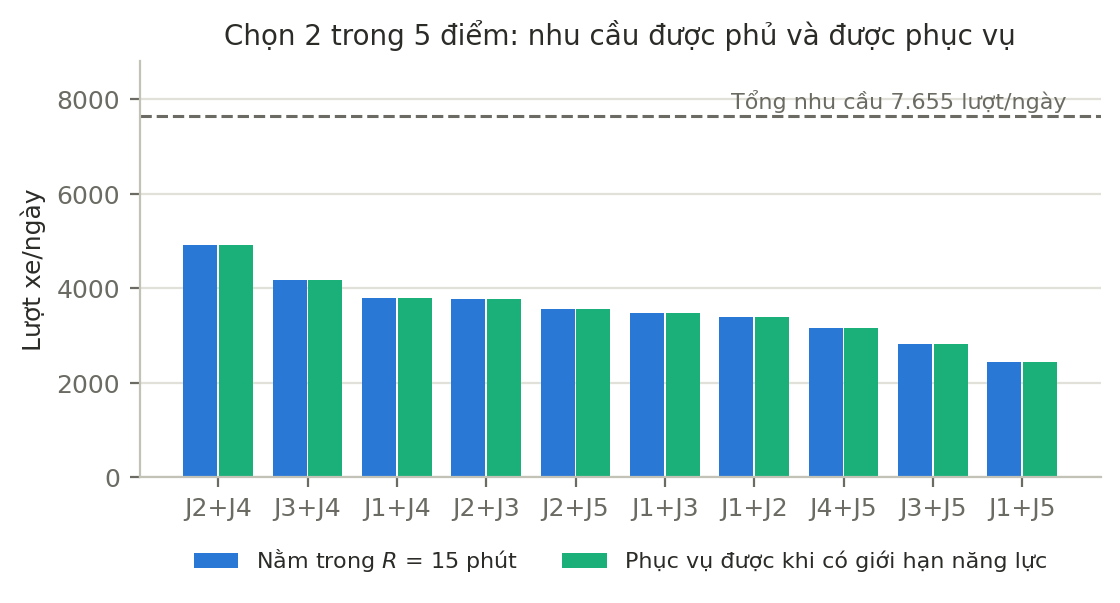
\includegraphics[width=0.9\linewidth]{figures/r2_location.png}
\caption{Nhu cầu nằm trong ngưỡng $R$ và nhu cầu phục vụ được của mười tổ hợp.}
\label{r2:loc-fig}
\source{\texttt{analysis/extension\_analysis.py}; dân số 2019, các tham số còn lại là ước tính/giả định}
\end{figure}

\textbf{Hai mục tiêu cho hai câu trả lời.} Theo mục tiêu (a), \textbf{J2 Đống Đa +
J4 Hoàng Mai} phục vụ 4\,916 lượt/ngày (64,2\% nhu cầu); J2 nhận Cầu Giấy, Đống
Đa, Thanh Xuân (2\,664 lượt/ngày, $\rho_{\max}=0{,}78$). Theo mục tiêu (b),
\textbf{J3 Hà Đông + J4 Hoàng Mai} lãi 163,2 triệu đồng/tháng so với 153,2 triệu
của J2 + J4, dù chỉ phục vụ 54,5\% nhu cầu: J2 nằm ở vùng giá thuê cao
(150 triệu đồng/tháng) và phải gánh tải gần năng lực. Một doanh nghiệp tư nhân
chịu áp lực chiết khấu thấp sẽ chọn (b); nếu mục tiêu là độ phủ dịch vụ (ví
dụ cam kết với đầu mối về sản lượng), (a) phù hợp hơn.

\exttable{tab_ext_location_sens.tex}{Độ nhạy của quyết định định vị}{r2:loc-sens}
\textbf{Độ bền.} J3 + J4 là tổ hợp lãi nhất ở 5/6 tình huống: $R=15$ hoặc 20
phút, nhu cầu giảm 20\% (KB-A), tăng 20\% (KB-B) và cửa hàng chỉ có 6 vòi; khi
nhu cầu tăng 20\%, J3 + J4 còn trở thành phương án phục vụ nhiều nhất vì J2 bị
giới hạn năng lực. Ngược lại, lợi nhuận của J2 + J4 giảm còn 73,6 triệu khi
nhu cầu giảm 20\% và còn 18,9 triệu nếu chỉ có 6 vòi. Chỉ khi $R=12$ phút (khách
rất ngại đi xa) thì tối ưu lợi nhuận chuyển sang J4 + J5.

\exttable{tab_ext_location_econ.tex}{Độ nhạy lợi nhuận BT2 theo lãi gộp (G) và chi phí cố định $f_j$ (G); số lượt phục vụ của từng tổ hợp giữ nguyên}{r2:loc-econ}
\textbf{Điều kiện kinh tế.} Hai tham số quyết định mục tiêu (b) đều là giả định:
lãi gộp 1\,500 đồng/lít và chi phí cố định $f_j$. Bảng~\ref{r2:loc-econ} tính
lại lợi nhuận khi thay đổi hai tham số này. Số lượt phục vụ không phụ thuộc vào
chúng nên giữ nguyên. Lãi gộp hòa vốn là 1\,098 đồng/lít với J3 + J4 và 1\,180
đồng/lít với J2 + J4. Ở mức 700 đồng/lít, ngưỡng bù chi phí mà~\cite{chietkhau}
nêu, mỗi lượt chỉ đóng góp 106 đồng và không tổ hợp nào có lãi. Ở mức 1\,000
đồng/lít cũng vậy. Ngay cả khi có lãi, lựa chọn giữa J2 và J3 vẫn đảo chiều:
J2 + J4 lãi hơn khi lãi gộp đạt 2\,000 đồng/lít hoặc khi $f_j$ giảm 30\%,
còn J3 + J4 lãi hơn khi $f_j$ tăng 30\%. Kết luận BT2 vì vậy có ba phần.
(i) \textbf{Chỉ mở thêm cửa hàng khi lãi gộp thực tế đạt trên khoảng 1\,100
đồng/lít.} (ii) \textbf{J4 Hoàng Mai} có mặt trong mọi phương án lãi nhất (Bảng~\ref{r2:loc-sens} và~\ref{r2:loc-econ}).
(iii) Điểm thứ hai là J3 Hà Đông nếu ưu tiên lợi nhuận ở mức cơ sở, hoặc J2
Đống Đa nếu ưu tiên độ phủ hay giá thuê thấp hơn giả định. Cần lấy lãi gộp
thật và báo giá thuê của từng điểm trước khi quyết định.
\todo{2}{Thay tọa độ xấp xỉ bằng địa chỉ ứng viên thật và thời gian đi lại từ
bản đồ số; kiểm tra lại số cửa hàng đối thủ trong bán kính $R$ để hiệu chỉnh thị phần 2\%.}

\subsection{Dự báo lượt xe ngày tới bằng học máy}
\label{r2:forecast}
Lịch theo giờ (BT1) chỉ tốt khi biết trước $\lambda_t$. Nhu cầu xăng có các
biến động \emph{biết trước được}: giá điều chỉnh có hiệu lực lúc 15 giờ, phần
lớn vào thứ Năm (các kỳ 22/10, 29/10, 5/11, 12/11/2026), đôi khi có kỳ bổ sung
giữa tuần (31/10, 3/11/2026)~\cite{moit2026,moit2026b}. Khi giá tăng, khách đổ
trước 15 giờ; khi giá giảm, khách chờ sau 15 giờ. Các biến động khác là tuần trước
Tết và kỳ nghỉ Tết, và tín hiệu căng thẳng nguồn cung. Nhóm dựng lịch sử 2 năm
(25/11/2024--22/11/2026) với \emph{lịch sự kiện thật}: Tết Ất Tỵ 29/1/2025, Tết
Bính Ngọ 17/2/2026, đợt cửa hàng đóng cửa giữa 2025 và đợt 17 cửa hàng tạm
dừng bán đầu tháng 3/2026~\cite{vtc2026}; biên độ điều chỉnh giá theo tuần lấy
quanh mức của các kỳ gần đây (E10RON95-III giảm 2\,075 đồng/lít ngày 5/11 và
1\,311 đồng/lít ngày 12/11/2026~\cite{moit2026b,moit2026}). Lượt xe
trong lịch sử là mô phỏng. Mô hình học máy là hồi quy Poisson (GLM, ước lượng IRLS):
\begin{multline}
\log\lambda_{d,h}=\beta_h+\gamma_{\text{thứ}(d)}+\delta_1\sin\tfrac{2\pi d}{364}+\delta_2\cos\tfrac{2\pi d}{364}
+\tau_1 T^{\text{trước}}_d+\tau_2 T^{\text{nghỉ}}_d\\
+\pi_1\Delta p_d\mathbf 1_{h<15}+\pi_2\Delta p_d\mathbf 1_{h\ge15}+\pi_3\Delta p_{d-1}+\eta s_{d-1}+\kappa\ell_{d-1},
\end{multline}
với $\Delta p_d$ là mức điều chỉnh dự kiến (nghìn đồng/lít, tính được trước từ
giá thế giới), $s_{d-1}$ là tín hiệu nguồn cung hôm trước, $\ell_{d-1}$ là log tỷ
số lượt hôm trước so với trung bình 28 ngày. Học trên 23/12/2024--4/1/2026,
kiểm tra trên 84 ngày 5/1--29/3/2026 (có Tết và đợt tháng 3).
\exttable{tab_ext_ml_acc.tex}{Độ chính xác dự báo trên 84 ngày kiểm tra; ``ngày sự kiện'' là 25 ngày có Tết, điều chỉnh giá $\ge$1\,000 đồng/lít hoặc căng thẳng nguồn cung}{r2:ml-acc}
\begin{figure}[htbp]\centering
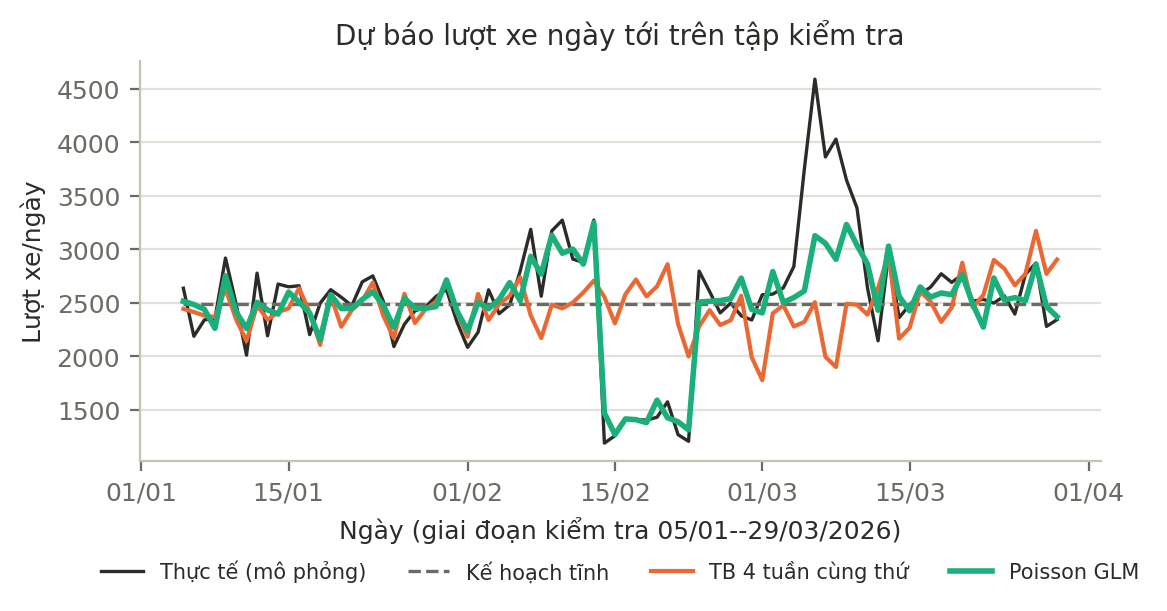
\includegraphics[width=0.9\linewidth]{figures/r2_forecast.png}
\caption{Dự báo tổng lượt xe/ngày trên tập kiểm tra.}\label{r2:ml-fig}
\source{\texttt{analysis/extension\_analysis.py}; lượt xe mô phỏng, lịch sự kiện theo thực tế}
\end{figure}
GLM giảm MAPE tổng ngày từ 18,33\% (kế hoạch tĩnh) và 19,63\% (trung bình 4 tuần
cùng thứ) xuống 7,25\%; trên 25 ngày sự kiện, từ khoảng 46\% xuống 10,44\%.
Trung bình 4 tuần thậm chí kém kế hoạch tĩnh vì nó ``nhớ'' Tết và đợt tháng 3
sang các tuần sau (Hình~\ref{r2:ml-fig}).

\textbf{Cần đọc kết quả này đúng mức.} Lịch sử lượt xe được mô phỏng với các
hiệu ứng do nhóm tự đặt: tuần trước Tết $\times1{,}20$, kỳ nghỉ Tết
$\times0{,}55$, mỗi nghìn đồng/lít tăng giá làm lượt xe trước 15 giờ tăng 25\%.
Mô hình ước lượng lại được gần đúng các giá trị này: $e^{0{,}167}=1{,}18$,
$e^{-0{,}540}=0{,}58$ và $e^{0{,}249}=1{,}28$. Điều đó chỉ cho thấy cách xây
biến và ước lượng là đúng: mô hình tìm lại được cấu trúc đã cài vào dữ liệu.
Đây \emph{không} phải bằng chứng về hành vi của khách thật. Cũng vì dữ liệu và
mô hình có cùng cấu trúc, MAPE 7,25\% là giới hạn trên lạc quan. Độ chính xác
thật chỉ biết được khi huấn luyện trên hóa đơn điện tử.
Giá trị vận hành của dự báo được đánh giá ở Mục~\ref{r3:ml-staff}.
\todo{2}{Huấn luyện lại trên dữ liệu hóa đơn điện tử thật; giữ cách chia theo
thời gian (không trộn ngẫu nhiên) và báo cáo MAPE theo tháng.}

}

\FloatBarrier
% \clearpage
% !TeX root = _main.tex
% ROLE 3: muc 7--9, giai phap, danh gia, thu nghiem va ket luan.
% Chi sua role cua minh va figures/rX_*. Khong sua tay bang do Python sinh.
% Nguoi ghep bai quan ly _main.tex va _content.tex.
% Macro Role*Supplement cuoi file giu ban nhap mo rong; KHONG duoc goi trong PDF.

\section{Phương án cải tiến và phân bổ nhân lực}
\label{r3:tobe}
\subsection{Từ hai nguyên nhân đến ba phương án}
Hai nguyên nhân đã chỉ ra ở Mục~\ref{r1:asis} và Mục~\ref{r2:diagnosis} dẫn
thẳng tới hai hướng cải tiến. Nguyên nhân thứ nhất là số kênh $c_t$ giữ cố
định trong khi lượng xe $\lambda_t$ thay đổi theo giờ. Nguyên nhân thứ hai là
thời gian phục vụ $E[S]$ dài vì việc trả tiền và lấy hóa đơn diễn ra ngay tại
trụ. Nhóm đưa mỗi hướng vào một phương án riêng để đo được tác động của từng
hướng (Bảng~\ref{r3:scenarios-design}).

\begin{table}[htbp]\centering\small
\caption{Ba phương án được so sánh trên cùng dòng xe đến mô phỏng}\label{r3:scenarios-design}
\begin{tabularx}{\linewidth}{@{}p{25mm}Y Y Y@{}}
\toprule
 & A0: AS-IS & A1: lịch theo giờ & A2: lịch theo giờ và trả trước \\
\midrule
Số kênh $c_t$ & 6 kênh ở mọi giờ & Theo BT1, dùng $E[S]$ hiện tại & Theo BT1, dùng $E[S]$ sau cải tiến \\
$E[S]$ (phút/xe) & Xe máy 1,5; ô tô 4,0 & Như A0 & Giảm 20\% (giả định): 1,2 và 3,2 \\
Thanh toán & Tiền mặt hoặc QR tại trụ & Như A0 & Trả trước trên ứng dụng; tiền mặt chỉ dùng khi lỗi \\
\bottomrule
\end{tabularx}
\end{table}

Cách đặt phương án như vậy giúp tách tác động theo từng bước. So A1 với A0
cho biết riêng việc xếp lịch theo giờ giúp được bao nhiêu, vì quy trình và
$E[S]$ giữ nguyên. So A2 với A1 cho biết rút ngắn thời gian phục vụ còn thêm
được gì. Tuy vậy, A2 đổi cả $E[S]$ lẫn lịch nên chưa tách được tác động riêng
của việc trả trước. Mức giảm 20\% cũng là giả định (G) trong
Bảng~\ref{r2:assumptions}, chưa có số đo.

\subsection{Lập lịch theo giờ (BT1)}
Lịch của A1 và A2 được lập bằng một bài toán, gọi tắt là BT1. Bài toán chọn
số kênh cho từng giờ sao cho chi phí nhân lực nhỏ nhất mà vẫn đạt mục tiêu về
thời gian chờ. Với chi phí $k=58\,000$ đồng cho một giờ nhân viên và 16 khung một
giờ từ 06:00 đến 22:00, bài toán được viết như sau:
\begin{align}
\min_{c_1,\ldots,c_{16}}\quad & k\textstyle\sum_{t=1}^{16}c_t \\
\text{với}\quad & c_t\in\{1,\ldots,8\},\ \rho_t<1,\ E[W_{q,t}]\le2\text{ phút},\ P(W_{q,t}>5)\le0{,}05. \nonumber
\end{align}
Ràng buộc đầu tiên giới hạn số kênh trong 8 vòi bơm. Ba ràng buộc còn lại
tính bằng M/M/c ở Mục~\ref{r2:method}: kênh không quá tải, chờ trung bình
không quá 2 phút và không quá 5\% số xe chờ trên 5 phút. Vì chi phí cộng
theo từng giờ và mỗi ràng buộc chỉ liên quan tới một giờ, lời giải là chọn
số kênh nhỏ nhất đạt yêu cầu ở từng giờ. Tỷ lệ bỏ đi không có trong công
thức M/M/c, nên được kiểm tra sau bằng mô phỏng (Mục~\ref{r3:evaluation}).

\resulttable{tab_shift_plan.tex}{Số kênh theo giờ của ba phương án (lời giải BT1)}{r3:staffing}

A1 không cần thêm người mà chỉ dời người sang giờ đông. Phương án này dùng
7 kênh ở ba giờ đông nhất (08--09, 17--18 và 18--19) và chỉ 4--5 kênh ở các
giờ vắng. Vì thế, lịch A1 cần 88 giờ nhân viên mỗi ngày thay vì 96. A2 chỉ
cần 72 giờ, vì khi $E[S]$ giảm 20\% thì mỗi kênh phục vụ được 47,8 xe mỗi
giờ thay vì 38,3 xe.

Thêm một kênh vào giờ đông có tác dụng rất lớn, vì hàng chờ tăng rất nhanh
khi $\rho$ gần 1. Tính bằng công thức M/M/c ở Mục~\ref{r2:method}, giờ 18--19 với 6
kênh có $\rho=0{,}98$ và thời gian chờ trung bình 12,2 phút. Với 7 kênh,
$\rho$ giảm còn 0,84 và thời gian chờ chỉ còn 0,8 phút.

BT1 mới chỉ cho biết số kênh cần ở mỗi giờ, chưa phải lịch làm việc. Để có lịch thật, cửa hàng còn phải ghép các giờ này
thành ca cho từng người, dài 4--8 giờ và có giờ nghỉ. Bước ghép ca
này chưa được tính trong báo cáo.

\subsection{Quy trình TO-BE và quy tắc vận hành}
Quy trình TO-BE của A2 giữ các bước chính của AS-IS nhưng đổi thứ tự trả
tiền (Hình~\ref{r3:bpmn}). Khách tạo đơn trên ứng dụng, chọn loại xăng và số
tiền trước khi vào trụ. Khi tới lượt, khách đưa mã đơn và xác nhận trả tiền.
Nhân viên chỉ bơm sau khi máy POS báo đã nhận tiền. Hóa đơn điện tử được gửi
thẳng về ứng dụng, nên xe không phải đứng chờ đếm tiền, thối tiền hay lấy
hóa đơn giấy. Khách không dùng ứng dụng vẫn đi theo luồng AS-IS ở
Hình~\ref{r1:bpmn}.

\begin{figure}[!htbp]\centering
\resizebox{\linewidth}{!}{%
\begin{tikzpicture}[
  mf/.style={{Circle[open,length=1.4mm]}-{Stealth[length=2.2mm,open]},dashed,thick,blue!50!black},
  mlab/.style={font=\scriptsize\itshape,fill=white,inner sep=1pt,text=blue!50!black},
  blab/.style={font=\scriptsize},
  gx/.style={diamond,draw,thick,fill=white,minimum width=9mm,minimum height=9mm,inner sep=0pt,font=\large},
  bbox/.style={draw,thick,fill=gray!12}]
\def\W{24.0}
% ---- Pool Khach hang ----
\draw[thick] (0,0) rectangle (\W,-2.4);
\draw[thick] (0.6,0) -- (0.6,-2.4);
\node[rotate=90,font=\scriptsize\bfseries] at (0.3,-1.2) {Khách hàng};
% ---- Pool Cua hang: 2 lan ----
\draw[thick] (0,-2.9) rectangle (\W,-8.3);
\draw[thick] (0.6,-2.9) -- (0.6,-8.3);
\draw (1.2,-2.9) -- (1.2,-8.3);
\draw (0.6,-5.6) -- (\W,-5.6);
\node[rotate=90,font=\scriptsize\bfseries] at (0.3,-5.6) {Cửa hàng xăng dầu};
\node[rotate=90,font=\scriptsize] at (0.9,-4.25) {Nhân viên bơm};
\node[rotate=90,font=\scriptsize] at (0.9,-6.95) {POS / HĐĐT};
% ---- Pool hop den ----
\draw[bbox] (0,-8.8) rectangle (17.0,-9.6);
\node[font=\scriptsize\bfseries] at (8.5,-9.2) {Ngân hàng / ví điện tử};
\draw[bbox] (17.5,-8.8) rectangle (\W,-9.6);
\node[font=\scriptsize\bfseries] at (20.75,-9.2) {Cơ quan thuế (hệ thống HĐĐT)};
% ---- Quy trinh khach hang ----
\node[ev] (cs) at (1.7,-1.5) {};
\node[blab,below=0mm of cs] {xe đến};
\node[task] (c1) at (3.75,-1.5) {Tạo đơn trên ứng dụng\\(loại xăng, số tiền)};
\node[gx] (cg) at (6.1,-1.5) {$\times$};
\node[blab,below=0.3mm of cg] {$\ge$20 xe chờ?};
\node[evend] (cb) at (7.4,-0.55) {};
\node[blab,anchor=west] at (7.7,-0.55) {bỏ đi; đơn chưa thu tiền tự hủy};
\node[task] (c2) at (9.0,-1.5) {Xếp hàng\\chờ tới lượt};
\node[task] (c3) at (11.7,-1.5) {Vào trụ,\\đưa mã đơn};
\node[task] (c4) at (14.6,-1.5) {Xác nhận trả tiền\\trên ứng dụng};
\node[task] (c5) at (21.6,-1.5) {Nhận hóa đơn trên\\ứng dụng, rời trụ};
\node[evend] (ce) at (23.45,-1.5) {};
\draw[flow] (cs) -- (c1);
\draw[flow] (c1) -- (cg);
\draw[flow] (cg.north) |- node[pos=0.3,left,blab]{có} (cb);
\draw[flow] (cg.east) -- node[above,blab]{không} (c2);
\draw[flow] (c2) -- (c3);
\draw[flow] (c3) -- (c4);
\draw[flow] (c4) -- (c5);
\draw[flow] (c5) -- (ce);
% ---- Lan nhan vien bom ----
\node[ev] (ss) at (7.7,-3.65) {};
\node[blab,below=0mm of ss] {trụ rảnh};
\node[task] (s1) at (10.0,-3.65) {Mời xe kế tiếp\\vào trụ};
\node[task] (s2) at (12.6,-3.65) {Quét mã đơn\\trên POS};
\node[task] (s3) at (17.4,-4.85) {Thu tại trụ như AS-IS\\(tiền mặt / QR)};
\node[task] (s4) at (19.9,-3.65) {Bơm đúng số tiền\\đã trả};
\draw[flow] (ss) -- (s1);
\draw[flow] (s1) -- (s2);
% ---- Lan POS / HDDT ----
\node[task] (p1) at (15.2,-7.0) {Chờ ngân hàng\\báo có};
\node[gx] (pg) at (17.4,-7.0) {$\times$};
\node[blab,anchor=north west] at ($(pg.south)+(0.05,-0.05)$) {Đã nhận tiền?};
\node[task] (p2) at (21.7,-7.0) {Xuất HĐĐT,\\gửi về ứng dụng};
\node[evend] (pe) at (23.45,-7.0) {};
\node[blab,anchor=south] at (pe.north) {xong};
\draw[flow] (s2.south) |- (p1.west);
\draw[flow] (p1) -- (pg);
\draw[flow] (pg.north) -- node[pos=0.45,left,blab,align=right]{không\\(lỗi, quá hạn)} (s3.south);
\draw[flow] (pg.east) -| node[pos=0.25,above,blab]{có} (s4.south);
\draw[flow] (s3.north) |- (s4.west);
\draw[flow] (s4.east) -| (p2.north);
\draw[flow] (p2) -- (pe);
% ---- Luong thong diep ----
\draw[mf] (10.85,-3.2) -- node[mlab]{lời mời} (10.85,-1.95);
\draw[mf] (12.3,-1.95) -- node[mlab]{mã đơn} (12.3,-3.2);
\draw[mf] (15.0,-1.95) -- node[mlab,pos=0.25]{xác nhận trả} (15.0,-6.55);
\draw[mf] (14.6,-7.45) -- node[mlab]{lệnh thu} (14.6,-8.8);
\draw[mf] (15.8,-8.8) -- node[mlab]{báo có} (15.8,-7.45);
\draw[mf] (22.5,-6.55) -- node[mlab,pos=0.6]{hóa đơn} (22.5,-1.95);
\draw[mf] (21.7,-7.45) -- node[mlab]{dữ liệu HĐ} (21.7,-8.8);
% ---- Moc do va ghi chu ----
\node[tmark] at (9.0,-2.15) {$a_i$: vào hàng};
\node[tmark] at (10.0,-4.35) {$b_i$: bắt đầu phục vụ};
\node[tmark] at (20.6,-2.15) {$d_i$: rời trụ};
\node[tmark,anchor=west,align=left] at (1.4,-3.55) {\textbf{A1:} số người đứng trụ theo\\lịch $c_t$ từng giờ (Bảng~\ref{r3:staffing})};
\node[tmark,anchor=west,align=left] at (1.4,-4.9) {\textbf{$S$ giảm (giả định 20\%):} không\\đếm tiền, thối tiền, giao hóa đơn giấy};
\node[tmark,anchor=west,align=left] at (1.4,-6.6) {\textbf{Ngoại lệ:} đã thu tiền mà không bơm\\được (vòi hỏng, hết xăng) thì hủy đơn,\\hoàn tiền; cuối ngày đối soát};
\end{tikzpicture}}
\caption{Quy trình TO-BE của A2: khách tạo đơn và trả tiền trước khi bơm, hóa đơn tự gửi về ứng dụng, số người đứng trụ theo lịch từng giờ. Ký pháp giống Hình~\ref{r1:bpmn}; khách không dùng ứng dụng vẫn đi theo luồng AS-IS.}
\label{r3:bpmn}
\source{nhóm vẽ bằng TikZ theo cùng ký pháp với hình AS-IS; Claude (Anthropic) hỗ trợ dựng mã hình; người viết role 3 kiểm tra ký pháp và luồng}
\end{figure}

Bảng~\ref{r3:changes} tóm tắt những gì thay đổi về vai trò, công nghệ và
chính sách phục vụ. Thay đổi lớn nhất về vai trò là khách tự làm phần đặt
yêu cầu và trả tiền, còn nhân viên chỉ tập trung vào việc bơm. Về chính sách,
số người đứng trụ không còn cố định mà đi theo lượng xe từng giờ.

\begin{table}[htbp]\centering\small
\caption{Những gì thay đổi từ AS-IS sang TO-BE}\label{r3:changes}
\begin{tabularx}{\linewidth}{@{}p{23mm}Y Y p{27mm}@{}}
\toprule
Thành phần & AS-IS & TO-BE & Người phụ trách \\
\midrule
Số người đứng trụ & 6 người ở mọi giờ & Theo lịch $c_t$ của BT1; lập lại khi lượng xe đổi rõ & Cửa hàng trưởng \\
Đặt yêu cầu & Khách nói loại xăng và số tiền tại trụ & Khách tạo đơn trên ứng dụng trước khi vào trụ & Khách \\
Thanh toán & Sau khi bơm, bằng tiền mặt hoặc QR & Trước khi bơm, qua ví hoặc ngân hàng; tiền mặt chỉ dùng khi lỗi & POS, nhân viên bơm \\
Hóa đơn & Nhân viên giao tại trụ & Tự gửi về ứng dụng & POS / HĐĐT \\
Xử lý lỗi & QR lỗi thì thu lại tiền mặt & Báo có lỗi thì thu như AS-IS; đã thu mà không bơm được thì hoàn tiền & Nhân viên; cửa hàng trưởng đối soát \\
\bottomrule
\end{tabularx}
\end{table}

Quy trình mới cần thêm vài quy tắc để không sinh lỗi mới. Đơn chỉ là đơn
nháp, chưa thu tiền cho tới khi xe vào trụ, nên khách bỏ hàng thì đơn tự hủy.
Hai tình huống lỗi còn lại được xử lý như ở dòng cuối Bảng~\ref{r3:changes}.
Cuối ngày, cửa hàng trưởng đối soát, tức là kiểm tra số tiền đã thu có khớp
với lượng xăng đã bơm hay không.

TO-BE cũng có những đánh đổi cần tính trước. Lợi ích của A2 phụ thuộc vào số
khách chịu dùng ứng dụng; nếu ít người dùng, $E[S]$ sẽ giảm ít hơn 20\%. Cửa
hàng phải trả chi phí ứng dụng và thanh toán, được giả định là 250 nghìn đồng
mỗi ngày, chưa kể chi phí đào tạo. Ngoài ra, cả A1 và A2 đều bớt người ở giờ
vắng, nên phần dự phòng khi có sự cố nhỏ hơn AS-IS (Mục~\ref{r3:scen3}).
\FloatBarrier

\section{Đánh giá, độ nhạy và giới hạn}
\label{r3:evaluation}
\subsection{So sánh trên cùng bộ chỉ số}
Bảng~\ref{r3:comparison} so sánh ba phương án trên cùng 20 ngày mô phỏng. Cả
ba phương án dùng chung một dòng xe đến, nên chênh lệch giữa các cột đến từ
phương án chứ không đến từ dữ liệu.

\resulttable{tab_comparison.tex}{Kết quả mô phỏng 20 ngày; ba phương án dùng chung dòng xe đến}{r3:comparison}

A1 giải quyết được vấn đề ở giờ cao điểm mà còn dùng ít giờ nhân viên hơn.
Trong khung 17--19, tỷ lệ xe chờ quá 5 phút giảm từ 6,18\% xuống 0,50\%, còn
tỷ lệ bỏ đi giảm từ 2,26\% xuống 0,17\%. Cả hai đều dưới ngưỡng 5\% và 1\%
đặt ra ở Mục~\ref{r1:scope}. Cùng lúc đó, lịch A1 cần ít hơn 8 giờ nhân viên mỗi
ngày, tương đương 464 nghìn đồng theo mô hình. Lý do là A1 chuyển người từ giờ vắng sang giờ
đông chứ không thêm người.

Cái giá của A1 là nhiều xe phải chờ một chút hơn ở giờ vắng. Tỷ lệ xe phải
chờ tăng từ 40,9\% lên 43,8\%, và mức sử dụng nhân viên tăng từ 67,9\% lên
74,5\%. Tuy vậy, các lần chờ này rất ngắn: 90\% số xe chờ không quá 1,51
phút, so với 2,37 phút ở A0. Như vậy, A1 đổi nhiều lần chờ rất ngắn để lấy
ít lần chờ dài.

A2 chủ yếu giúp tiết kiệm nhân lực chứ không giảm chờ thêm nhiều. Ở khung
17--19, thời gian chờ trung bình chỉ giảm từ 0,56 xuống 0,36 phút so với A1,
nhưng lịch A2 cần ít hơn 16 giờ nhân viên mỗi ngày. Sau khi trừ 250 nghìn đồng chi
phí công nghệ, A2 rẻ hơn A1 678 nghìn đồng và rẻ hơn A0 khoảng 1,14 triệu
đồng mỗi ngày. Đây chỉ là mức tiềm năng, vì nó dựa trên giả định $E[S]$ giảm
20\% và chưa tính chi phí chuyển đổi. Tính cả ngày, A2 còn có tỷ lệ chờ quá
5 phút (0,48\%) và lần chờ dài nhất (9,10 phút) cao hơn A1. Lý do là A2 ít
người hơn nên ít dư ra để đỡ những lúc xe dồn.

\subsection{Ba kịch bản: nhu cầu thấp, nhu cầu cao và thiếu người}
\label{r3:scen3}
Để xem các phương án có vững không, nhóm giữ nguyên lịch đã lập và thử ba
kịch bản. Hai kịch bản đầu đổi lượng xe đến: giảm 20\% (nhu cầu thấp) và tăng
20--40\% (nhu cầu cao). Kịch bản thứ ba là gián đoạn phục vụ do thiếu một
nhân viên. Mỗi cấu hình chạy 30 ngày với dòng xe đến khác
Bảng~\ref{r3:comparison}, nên mức cơ sở chênh nhẹ. Vì vậy chỉ nên so các
phương án trong cùng một bảng.

\resulttable{tab_sensitivity.tex}{Kết quả khi lượng xe đến thay đổi, giữ nguyên lịch (30 ngày mỗi cấu hình)}{r3:sensitivity}

Khi nhu cầu thấp, cả ba phương án đều đạt mục tiêu. Với lượng xe bằng 80\%
mức cơ sở, tỷ lệ chờ quá 5 phút của cả ba chỉ từ 0,01\% đến 0,12\%. Như vậy,
lịch theo giờ không gây hại khi vắng khách mà vẫn giữ được phần giờ công
tiết kiệm.

Khi nhu cầu cao, lịch đã lập nhanh chóng mất tác dụng. Với lượng xe tăng
20\%, A0 có 2,88\% khách bỏ đi, vượt ngưỡng 1\%. A1 vừa chạm ngưỡng với
0,95\%, vì giờ cao điểm đã có $\rho=1{,}01$. A2 còn dư hơn một chút với
0,53\%. Khi lượng xe tăng 40\%, cả ba đều không đạt, với 4,8--7,9\% khách bỏ
đi. Lúc này A1 thậm chí có tỷ lệ chờ quá 5 phút cao hơn A0 (14,81\% so với
10,83\%), vì A1 đã bớt người ở giờ vắng. Điều này cho thấy một lịch chỉ đúng
với mức nhu cầu dùng để lập nó, nên phải lập lại khi lượng xe thay đổi rõ.

\resulttable{tab_risk.tex}{Các tình huống rủi ro của A2 (30 ngày mỗi tình huống)}{r3:risks}

Thiếu người là rủi ro lớn nhất của các lịch đã bớt người. Khi A2 thiếu một nhân
viên ở mọi giờ, tỷ lệ chờ quá 5 phút tăng từ 0,48\% lên 16,71\% và 1,92\%
khách bỏ đi (Bảng~\ref{r3:risks}). Với A1, thiếu một người trong khung 17--19
sẽ đưa số kênh về 6, đúng như AS-IS. Theo Bảng~\ref{r2:hourly}, giờ 18--19
khi đó lại có $\rho=0{,}98$ và thời gian chờ trung bình khoảng 12 phút. Vì
vậy, cửa hàng cần một người dự phòng có thể gọi đến trong giờ cao điểm.

Rủi ro thứ hai của A2 là trả trước rút ngắn thời gian phục vụ ít hơn dự
kiến. Nếu chỉ giảm được 10\% thay vì 20\%, A2 vẫn đạt mục tiêu tính cả ngày,
với 1,45\% xe chờ quá 5 phút và 0,10\% khách bỏ đi. Tuy vậy, cần kiểm tra lại
từng giờ trước khi áp dụng.

\subsection{Độ nhạy theo các giả định chưa đo được}
Thời gian phục vụ, độ dao động của nó và ngưỡng bỏ đi đều là giả định (G)
trong Bảng~\ref{r2:assumptions}. Nhóm cho từng giả định lệch khỏi giá trị cơ
sở để xem kết luận có đổi không. Trong ba giả định này, $E[S]$ ảnh hưởng
mạnh nhất.

\resulttable{tab_sens_service.tex}{Kết quả khi $E[S]$ thực khác giả định ($\times$0,8--1,4), giữ nguyên lịch đã lập (30 ngày; $E[S]$ của A2 nhân cùng hệ số)}{r3:sens-service}

Nếu $E[S]$ thực dài hơn giả định mà lịch giữ nguyên, A1 sẽ không còn đạt mục
tiêu. Khi $E[S]$ dài hơn 20\% (xe máy 1,8 phút), A1 có 6,71\% xe chờ quá 5
phút và 1,00\% khách bỏ đi, dù vẫn tốt hơn A0 (11,53\% và 3,01\%). Khi dài
hơn 40\%, A1 còn kém A0 về tỷ lệ chờ quá 5 phút (38,58\% so với 29,34\%).
Ngược lại, nếu $E[S]$ ngắn hơn 20\%, cả ba phương án đều đạt.

\resulttable{tab_sens_replan.tex}{Giờ nhân viên cần nếu lập lại lịch theo $E[S]$ thực; ``không đạt'' là số giờ trong ngày không đạt mục tiêu dù mở đủ 8 vòi}{r3:sens-replan}

Nếu lập lại lịch theo $E[S]$ đo được, A1 vẫn dùng được nhưng sẽ chạm giới
hạn 8 vòi. Với $E[S]$ dài hơn 20\%, A1 cần 101 giờ nhân viên mỗi ngày thay vì
88, và vẫn có 1 giờ không đạt mục tiêu dù mở đủ 8 vòi. Với $E[S]$ dài hơn
40\%, A1 cần 114 giờ và có 3 giờ không đạt. Khi đó thêm người không còn giúp
được, vì đã hết vòi. A2 đạt mục tiêu ở mọi giờ trong cả bốn mức, kể cả mức
dài hơn 40\% (96 giờ nhân viên). Vì vậy, nếu $E[S]$ thực dài hơn giả định,
rút ngắn thời gian ở trụ trở thành điều kiện cần chứ không chỉ để tiết kiệm.

Hai giả định còn lại không làm đổi thứ tự giữa các phương án. CV là hệ số
biến thiên, bằng độ lệch chuẩn chia cho trung bình, cho biết thời gian phục
vụ dao động nhiều hay ít. Khi CV đi từ 0,5 đến 1,2, A1 luôn đạt mục tiêu, với
tỷ lệ chờ quá 5 phút không quá 0,84\%, và luôn tốt hơn A0. Ngưỡng bỏ đi chỉ
chuyển rủi ro qua lại giữa chờ lâu và mất khách. Với ngưỡng 10 xe, A0 mất
1,22\% khách; với ngưỡng 30 xe, A0 có 3,77\% xe chờ quá 5 phút. A1 đạt mục
tiêu ở cả hai trường hợp. Số liệu chi tiết nằm trong tệp
\texttt{tables/tab\_sens\_other.tex} của dự án.

Các kết quả độ nhạy cho thấy cách lập lịch theo $\lambda_t$ và $E[S]$ vẫn
đúng khi giả định lệch, nhưng số giờ công cụ thể phải tính lại từ $E[S]$ đo
thật. Do đó, việc bấm giờ thời gian phục vụ theo Phụ lục~\ref{r2:app-plan}
cần làm trước khi áp dụng lịch.

\subsection{Giới hạn}
Các kết quả trên đến từ mô hình nên còn bốn giới hạn chính. Lượt xe đến và
thời gian phục vụ là số mô phỏng; quy mô được hiệu chỉnh từ số liệu công bố
nhưng chưa đo tại cửa hàng nào. Mô hình coi mọi vòi phục vụ được mọi loại
xe, trong khi thực tế thường có trụ riêng cho ô tô. Ngưỡng bỏ đi 20 xe và mức
giảm 20\% thời gian phục vụ là giả định. Cuối cùng, mỗi ngày mô phỏng bắt đầu
với hàng rỗng, và ở tải rất cao kết quả mô phỏng lệch xa công thức
(Mục~\ref{r2:diagnosis}). Vì vậy, số liệu của giờ 18--19 chỉ nên xem là ước
lượng.

\section{Đề xuất triển khai và kết luận}
\label{r3:conclusion}
\subsection{Áp dụng lịch theo giờ trước, thử trả trước sau}
Nhóm đề xuất áp dụng A1 trước và chỉ thử A2 khi đã có số đo. Theo quy tắc
chọn ở Mục~\ref{r1:scope}, phương án được chọn phải đạt các ngưỡng, có chi
phí hợp lý và xếp được thành ca. A1 đạt các ngưỡng ở cả ngày lẫn giờ cao điểm,
rẻ hơn AS-IS và không cần thêm công nghệ. Riêng điều kiện xếp được thành ca
chưa được kiểm tra, nên đây là việc đầu tiên khi thử lịch (Bảng~\ref{r3:pilot}). A2 rẻ hơn nữa trong mô hình, nhưng lợi ích
dựa trên mức giảm 20\% chưa đo được, cần khách dùng ứng dụng và có ít dự
phòng khi thiếu người.

Khi áp dụng A1, cửa hàng cần thêm hai quy tắc vận hành. Thứ nhất, luôn có
một người dự phòng có thể gọi đến trong khung 17--19, vì thiếu một người ở
giờ này đưa cửa hàng về đúng tình trạng AS-IS. Thứ hai, lịch phải được lập
lại khi lượng xe giờ đông tăng gần 20\%, là mức mà lịch A1 vừa chạm ngưỡng
bỏ đi (Mục~\ref{r3:scen3}). Bảng~\ref{r3:pilot} nêu các bước thử trước khi
áp dụng rộng.

\begin{table}[htbp]\centering\small
\caption{Kế hoạch kiểm tra giải pháp trước khi áp dụng rộng}\label{r3:pilot}
\begin{tabularx}{\linewidth}{@{}p{24mm}Y Y@{}}
\toprule
Bước & Việc cần làm và người phụ trách & Tiêu chí quyết định \\
\midrule
Đo hiện trạng & Cửa hàng trưởng tổ chức ghi lượt đến, lượt bỏ đi và các mốc $a_i,b_i,d_i$ theo giờ; bấm giờ 30--50 lượt cho mỗi loại xe. Hóa đơn điện tử chỉ cho số lượt bán theo giờ, không cho giờ xe đến hay lượt bỏ đi. & Có số liệu cả giờ vắng và giờ đông; tách được thời gian bơm và thời gian trả tiền. \\
Thử lịch A1 & Ghép số kênh theo giờ thành ca có giờ nghỉ; thử trên các ngày cùng thứ, có lượng xe tương đương. & Tỷ lệ chờ quá 5 phút và tỷ lệ bỏ đi giờ đông giảm; ghi lại giờ công và chi phí thực. \\
Thử A2 ở phạm vi nhỏ & Cho một nhóm khách tạo đơn và trả trước; vẫn giữ cách trả tiền tại trụ. & Thời gian từ lúc vào trụ đến lúc rời trụ giảm; lỗi giao dịch không tăng; lợi ích đủ bù chi phí. \\
Rà soát định kỳ & Cửa hàng trưởng theo dõi số liệu theo giờ, ghi nhận nhu cầu tăng, người vắng và vòi hỏng. & Nếu vượt ngưỡng thì gọi người dự phòng hoặc lập lại lịch; không cố giữ mức tiết kiệm đã định. \\
\bottomrule
\end{tabularx}
\end{table}

\subsection{Kết luận}
Câu trả lời cho câu hỏi chính ở Mục~\ref{r1:scope} là có, trong phạm vi mô
hình. Chỉ cần xếp số nhân viên theo giờ (A1), tỷ lệ xe chờ quá 5 phút trong
khung 17--19 giảm từ 6,18\% xuống 0,50\% và tỷ lệ bỏ đi từ 2,26\% xuống
0,17\%, đều dưới ngưỡng. Trong khi đó, lịch tính toán chỉ cần 88 thay vì 96
giờ nhân viên mỗi ngày, dù con số này còn phải ghép thành ca và thử tại cửa
hàng. Cải tiến khâu thanh toán (A2) không cần để đạt ngưỡng ở kịch bản
cơ sở. Nó chủ yếu giúp tiết kiệm thêm nhân lực, và trở thành điều kiện cần
nếu thời gian phục vụ thực dài hơn giả định.

Đây là đề xuất dựa trên mô hình, chưa được kiểm chứng tại cửa hàng. Bước
tiếp theo là bấm giờ thời gian phục vụ, thử A1 trong một số ngày và chỉ mở
rộng khi các ngưỡng vẫn đạt; trả trước chỉ nên đầu tư khi đo được lợi ích.
\todo{3}{Chốt lịch ca khả thi, chi phí thực và kết quả thử nghiệm với cửa hàng;
không trình bày kết quả mô phỏng như thành tích đã triển khai.}

\newcommand{\RoleThreeSupplement}{%
\section{Kịch bản chiến lược và trải nghiệm khách hàng}
\label{r3:scenarios}
\subsection{Ba kịch bản tương lai và hai lựa chọn chiến lược}
Từ PESTEL (Bảng~\ref{r1:pestel}), nhóm xây ba kịch bản cho cửa hàng ở tầm
12--24 tháng. Xác suất chỉ dùng để tính chi phí kỳ vọng; tiêu chí chính là
hối tiếc tối đa, không phụ thuộc xác suất.
\begin{itemize}
\item \textbf{KB-A -- Nhu cầu thấp} (0,30): lượt xe $\times0{,}8$ do vùng phát
thải thấp mở rộng và khách chuyển sang xe điện~\cite{ct20,lez2026}.
\item \textbf{KB-B -- Nhu cầu tăng} (0,45): lượt xe $\times1{,}2$ do cửa hàng lân
cận đóng cửa vì chiết khấu thấp~\cite{chietkhau} và xe máy mới tăng~\cite{reg2025}.
\item \textbf{KB-C -- Gián đoạn} (0,25): như đợt tháng 3/2026~\cite{vtc2026},
khách dồn sang ($\times1{,}35$) và bán có kiểm soát làm thời gian phục vụ tăng 15\%.
\end{itemize}
Lựa chọn \textbf{CL-A -- nhân lực theo lịch, không số hóa} giữ lịch A1 (88 giờ).
Lựa chọn \textbf{CL-B -- số hóa} có hai biến thể: \emph{tĩnh} giữ lịch A2 (72 giờ);
\emph{thích ứng} dùng dự báo (Mục~\ref{r2:forecast}) để tối ưu lại $c_t$ theo
BT1 mỗi ngày, phần giờ vượt lịch A2 do nhân viên bán thời gian đảm nhận với đơn
giá $1{,}5\times58\,000$ đồng/giờ. Mỗi ô mô phỏng 30 ngày, cùng seed trong một
kịch bản.

\subsection{Mô hình mất khách theo thế hệ}
\label{r3:cx}
Mục tiêu dài hạn của chiến lược là khách quay lại, không bỏ cửa hàng. Một khách
thuộc phân khúc $g$ đã chờ $w$ phút có xác suất không hài lòng đến mức lần sau
bỏ đi là
\begin{equation}
p_g(w)=1-\exp\!\left[-(w/\theta_g)^2\right],
\end{equation}
dạng Weibull để chờ ngắn gần như không gây mất khách còn chờ dài làm xác suất
tăng nhanh; khách bỏ đi vì hàng dài có $p=1$. Mỗi lượt mất gây thiệt hại
$p\times[\text{lãi gộp lượt đó}+c_g\times\text{CLV}]$, với $c_g$ là xác suất
chuyển hẳn sang cửa hàng khác. CLV là lãi gộp 3 năm của một khách quen: xe máy
$73\times2{,}5\times1\,500\times3\approx820$ nghìn đồng, ô tô
$52\times30\times1\,500\times3\approx7{,}02$ triệu đồng. Các giá trị $\theta_g$,
$c_g$ trong Bảng~\ref{r3:segments} là giả định để thể hiện cơ chế, chưa có khảo sát.
\exttable{tab_ext_segments.tex}{Tỷ lệ mất khách theo phân khúc trong KB-B; $\theta_g$, $c_g$ là giả định}{r3:segments}
\textbf{Nhận định.} Với cùng một hàng chờ, Gen Z mất 8,79\% ở A0 so với 4,77\%
ở nhóm 60+. Khi chờ đã ngắn (CL-B thích ứng), khoảng cách tương đối còn lớn
hơn (1,41\% so với 0,50\%, gấp 2,8 lần): nhóm trẻ --- nhiều người là sinh viên
và tài xế giao hàng --- là nhóm đầu tiên rời đi và cũng là nhóm chuyển sang xe
điện sớm nhất. Hàm ý: thông báo thời gian chờ dự kiến và trả trước trên ứng
dụng cho nhóm trẻ; giữ thu tiền mặt và nhân viên hỗ trợ cho nhóm lớn tuổi.

\subsection{Kết quả theo kịch bản}
\exttable{tab_ext_scenarios.tex}{Hiệu quả của các chiến lược trong ba kịch bản; chi phí và giá trị mất tính bằng nghìn đồng/ngày}{r3:scen-table}
\begin{figure}[htbp]\centering
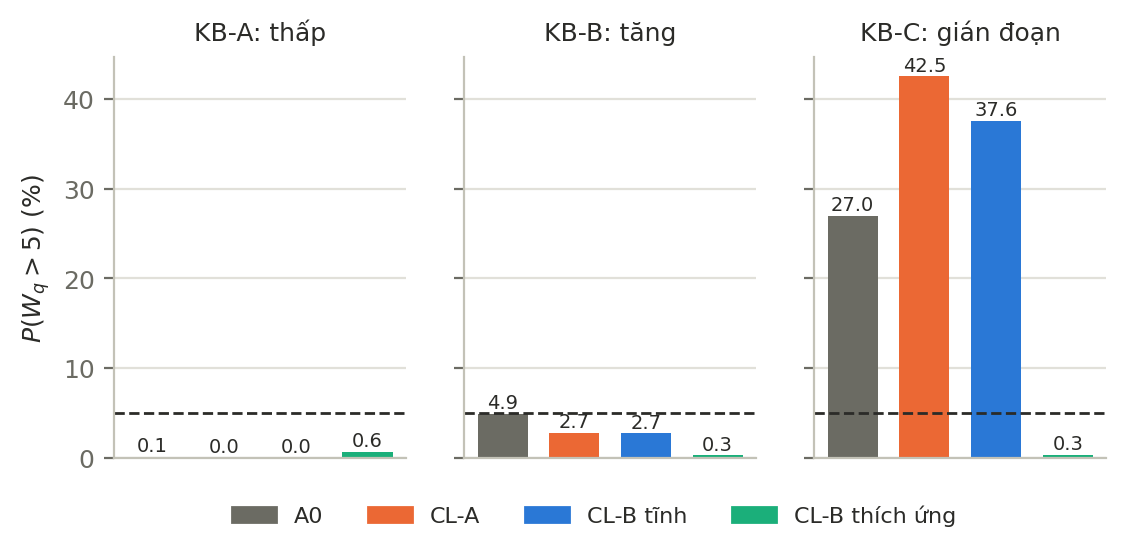
\includegraphics[width=0.92\linewidth]{figures/r3_scenarios.png}
\caption{Tỷ lệ xe chờ quá 5 phút theo kịch bản; đường đứt là mục tiêu 5\%.}
\label{r3:scen-fig}
\source{\texttt{analysis/extension\_analysis.py}; dữ liệu mô phỏng}
\end{figure}
(1) Ở KB-A mọi lựa chọn đều đạt; CL-B tĩnh rẻ nhất (4,68 triệu đồng/ngày) vì
biến thể thích ứng cắt xuống 59 giờ và làm chờ tăng nhẹ. (2) Ở KB-B, lịch tĩnh
vẫn đạt $P(W_q{>}5)\le5\%$ nhưng 3,6--4,4\% khách bị mất; CL-B thích ứng tăng lên
81 giờ và chỉ mất 0,98\%. (3) KB-C quyết định lựa chọn: mọi lịch tĩnh đều sụp
(37,6--42,5\% xe chờ quá 5 phút, 11,8--13,6\% bỏ đi), trong khi CL-B thích ứng
giữ 0,30\% với 101 giờ/ngày --- gần chạm giới hạn 8 vòi ở giờ cao điểm.
\exttable{tab_ext_regret.tex}{Tổng chi phí (nghìn đồng/ngày), kỳ vọng và hối tiếc tối đa; ``đạt'' khi $P(W_q{>}5)\le5\%$ và bỏ đi $\le1\%$}{r3:regret}

\subsection{Đánh giá và quyết định}
Nhóm chọn \textbf{CL-B thích ứng}: hối tiếc tối đa chỉ 554,8 nghìn đồng/ngày
(ở KB-A) so với 59--66 triệu đồng/ngày của hai lựa chọn tĩnh (ở KB-C); chi phí kỳ
vọng 7,31 so với 23,90--26,72 triệu đồng/ngày; và là lựa chọn duy nhất đạt mục
tiêu ở cả ba kịch bản.
\exttable{tab_ext_clv.tex}{Chi phí kỳ vọng (nghìn đồng/ngày) theo hệ số CLV}{r3:clv}
\textbf{Kết luận có bền không?} Ngay cả khi bỏ hoàn toàn giá trị khách quay lại
(CLV = 0, chỉ tính lãi gộp của lượt bị mất), CL-B thích ứng vẫn rẻ nhất
(5,34 so với 5,87 và 6,71 triệu đồng/ngày) vì khách bỏ đi trong KB-C là doanh
thu mất ngay. Điều kiện để kết luận đúng là \emph{dự báo đủ tốt} và \emph{có
nguồn nhân viên bán thời gian huy động được trong ngày}.

\subsection{Năng lực thích ứng nhờ dự báo}
\label{r3:ml-staff}
Mô hình GLM ở Mục~\ref{r2:forecast} được dùng để lập lịch $c_t$ cho từng ngày
kiểm tra; mỗi ngày được mô phỏng với nhu cầu thật của ngày đó.
\exttable{tab_ext_ml_staff.tex}{Lập lịch theo dự báo trên 84 ngày kiểm tra (5/1--29/3/2026); ngày vi phạm: $P(W_q{>}5)>5\%$ hoặc bỏ đi $>1\%$}{r3:ml-staff-table}
Lịch A2 tĩnh vi phạm ở 16,7\% số ngày và 10,67\% xe chờ quá 5 phút trong các
ngày sự kiện. Lịch theo GLM giảm số ngày vi phạm xuống 6,0\% mà chỉ dùng 70,48
giờ/ngày --- ít hơn lịch tĩnh. Phương án ``đệm 20\%'' đạt kết quả tương đương
(7,1\% ngày vi phạm) nhưng tốn 81 giờ/ngày; GLM tiết kiệm 10,5 giờ, tức 610
nghìn đồng/ngày (khoảng 18 triệu đồng/tháng). Lịch theo trung bình 4 tuần còn
kém lịch tĩnh (27,4\% ngày vi phạm) vì phản ứng trễ với sự kiện.

\begin{table}[htbp]\centering\small
\caption{Kế hoạch ứng phó: dấu hiệu sớm, ngưỡng kích hoạt và hành động}\label{r3:playbook}
\begin{tabularx}{\linewidth}{@{}p{14mm}Y Y Y@{}}
\toprule
Kịch bản & Dấu hiệu sớm & Ngưỡng kích hoạt & Hành động \\
\midrule
KB-A & Lượt xe dự báo giảm; vùng phát thải thấp mở rộng & $<2\,000$ lượt/ngày trong 4 tuần & Giảm kênh lúc vắng; đàm phán lắp tủ đổi pin/trạm sạc~\cite{vgx} \\
KB-B & Cửa hàng lân cận đóng cửa; dự báo tăng & $>2\,900$ lượt/ngày hoặc $\rho_{17-19}>0{,}85$ & Tối ưu lại $c_t$ ($\approx$81 giờ/ngày); tuyển thêm nhân viên bán thời gian \\
KB-C & Tin căng thẳng nguồn cung; điều chỉnh giá lớn & Tín hiệu nguồn cung hoặc $|\Delta p|\ge1\,000$ đồng/lít & Mở đủ 8 vòi giờ cao điểm; gọi ca dự phòng; hiển thị ETA, ưu tiên khách trả trước \\
\bottomrule
\end{tabularx}
\end{table}

\begin{table}[htbp]\centering\small
\caption{Học máy trong dịch vụ: tác động, chỉ số chấp nhận và kiểm soát}\label{r3:ml-uses}
\begin{tabularx}{\linewidth}{@{}p{27mm}Y Y Y@{}}
\toprule
Ứng dụng & Tác động lên mô hình & Chỉ số chấp nhận & Kiểm soát \\
\midrule
Dự báo lượt xe (đã thử) & $\hat\lambda_{d,h}\to c_t$ & MAPE $\le10\%$; ngày vi phạm $\le7\%$ & Cửa hàng trưởng duyệt lịch hằng ngày \\
Ước lượng độ kiên nhẫn & $\theta_g$ từ tỷ lệ bỏ đi theo độ dài hàng & Sai số dự báo bỏ đi & Chỉ dùng dữ liệu ẩn danh, gộp \\
Dự báo rời bỏ & Khách quen giảm tần suất & AUC; tỷ lệ giữ chân & Ưu đãi có đồng ý của khách \\
Phát hiện bất thường & Lượt bán đột biến, lỗi cột bơm & Thời gian phát hiện & Kiểm tra thủ công trước khi xử lý \\
\bottomrule
\end{tabularx}
\end{table}


}

\FloatBarrier
% \clearpage

\phantomsection
\addcontentsline{toc}{section}{Tài liệu tham khảo}
% Nguon bao chi/van ban duoc tim ngay 21/11/2026; nhom can mo lai tung nguon de kiem chung.
\bibliographystyle{unsrtnat}
\bibliography{reference} % nguon nam trong reference.bib, tu sap theo thu tu trich dan
% Them nguon hoc thuat SAU KHI da doc/kiem chung; khong tu dien DOI/nam/tac gia.

\appendix
\section{Phân công và cách ghép báo cáo}
\label{app:roles}
\begin{table}[H]\centering\small
\caption{Phân công theo role; mỗi người chịu trách nhiệm một file nội dung}
\begin{tabularx}{\linewidth}{@{}p{30mm}Y Y@{}}
\toprule
Người phụ trách & Nội dung chịu trách nhiệm & Đầu ra bàn giao \\
\midrule
Phạm Tuấn Anh & Vấn đề, phạm vi, khung hệ thống, bản đồ nguồn lực, bên liên quan, Blueprint và quy trình AS-IS. & Mục 1--4; vẽ Hình~\ref{r1:resource-map} và Hình~\ref{r1:bpmn}. \\
Đoàn Văn Tuyền & Dữ liệu, giả định, M/M/c, mô phỏng, kiểm chứng, phân tích nguyên nhân và mô hình mở rộng. & Mục 5--7 và Phụ lục~\ref{r2:appendix}. \\
Phạm Nam Khánh & Giải pháp, TO-BE, đối chứng, độ nhạy, rủi ro, kế hoạch thử nghiệm và kết luận. & Mục 8--10. \\
\bottomrule
\end{tabularx}
\end{table}
Phạm Tuấn Anh lập kế hoạch, chia role và rà soát lần cuối toàn bộ báo cáo;
cũng là người ghép bài, quản lý \texttt{\_main.tex}, \texttt{\_content.tex} và
nguồn trích dẫn. Mỗi người chỉ sửa file role của mình; các thay đổi chạm vào
role khác được thống nhất trước khi ghép.

% !TeX root = _main.tex
% ROLE 2 -- PHU LUC: bieu mau va ke hoach thu thap du lieu thuc (Batch 1, TV2).
% Duoc \input trong phan \appendix cua _content.tex. Nhan bat dau bang r2:.

\section{Biểu mẫu và kế hoạch thu thập dữ liệu thực}
\label{r2:app-plan}
Các tham số G và E trong Bảng~\ref{r2:assumptions} cần được đo lại. Phụ lục này
mô tả dữ liệu cần thu, cách thu và cách nạp vào mã phân tích.

\subsection{Hai nguồn dữ liệu}
\begin{enumerate}
\item \textbf{Hóa đơn điện tử (nguồn chính cho $\lambda_t$).} Mỗi lần bán xăng
đều có hóa đơn điện tử kèm dấu thời gian~\cite{nd70}. Nhóm đề nghị một cửa hàng
cung cấp bản trích xuất \emph{đã ẩn danh}: thời điểm xuất hóa đơn, số lít và
mặt hàng, trong tối thiểu 4 tuần liên tiếp có ít nhất một kỳ điều chỉnh giá.
Từ đó đếm được số lượt theo giờ và theo ngày.
\item \textbf{Bấm giờ tại chỗ (nguồn cho $E[S]$, CV, bỏ đi).} Hóa đơn chỉ cho
biết thời điểm thanh toán. Nó không cho biết lúc xe vào hàng chờ ($a_i$), lúc
bắt đầu bơm ($b_i$) hay số xe bỏ đi. Vì vậy hai người quan sát ghi theo Bảng~\ref{r2:form}.
\end{enumerate}

\begin{table}[htbp]\centering\small
\caption{Biểu mẫu bấm giờ; mỗi dòng là một lượt xe. Tên cột trùng với \texttt{data/requests\_asis\_simulated.csv}}
\label{r2:form}
\begin{tabularx}{\linewidth}{@{}p{39mm}p{24mm}Y@{}}
\toprule
Cột & Đơn vị / mã & Cách ghi \\
\midrule
\texttt{data\_label} & \texttt{OBSERVED} & Phân biệt với \texttt{SIMULATED} khi gộp dữ liệu \\
\texttt{day}, \texttt{hour\_slot} & ngày; \texttt{07-08} & Ngày quan sát và khung giờ \\
\texttt{vehicle\_id} & số thứ tự & Không ghi biển số \\
\texttt{vehicle\_class} & Xe máy / Ô tô & \\
\texttt{t\_arrival\_min} & phút từ 06:00 & $a_i$: lúc xe dừng vào cuối hàng chờ \\
\texttt{t\_service\_start\_min} & phút từ 06:00 & $b_i$: lúc nhân viên cầm vòi bơm \\
\texttt{t\_service\_end\_min} & phút từ 06:00 & $d_i$: lúc xe rời trụ sau khi thanh toán \\
\texttt{balked} & 0/1 & 1 nếu xe đến, thấy hàng dài và bỏ đi \\
\texttt{servers\_active} & số người & Số nhân viên đang bơm khi xe đến (thêm mới) \\
\texttt{payment} & TM / QR / thẻ / ứng dụng & Hình thức thanh toán (thêm mới) \\
\bottomrule
\end{tabularx}
\source{Nhóm đề xuất; \texttt{service\_min} và \texttt{wait\_min} được tính từ ba mốc thời gian}
\end{table}

\subsection{Lịch quan sát và cỡ mẫu}
\begin{itemize}
\item \textbf{Khung giờ:} 07--09, 11--13 và 17--19 của 2 ngày thường; thêm 1 thứ
Năm có kỳ điều chỉnh giá (quan sát 14--16 giờ) và 1 ngày cuối tuần.
\item \textbf{Cỡ mẫu:} tối thiểu 30--50 lượt có đủ $a_i,b_i,d_i$ cho mỗi loại xe
trong mỗi khung giờ. Ô tô ít (khoảng 2,7\% lượt), nên ghi mọi ô tô đến.
\item \textbf{Phân công:} người thứ nhất ghi $a_i$ và số xe bỏ đi ở đầu hàng;
người thứ hai ghi $b_i,d_i$ tại các trụ. Hai người dùng chung một đồng hồ, ví
dụ ứng dụng bấm giờ trên điện thoại đã đồng bộ.
\end{itemize}

\subsection{Kiểm tra và nạp vào mô hình}
\begin{enumerate}
\item \textbf{Dòng đến:} đếm số xe theo khoảng 15 phút. Nếu tỷ số phương sai/trung
bình gần 1 thì giả định Poisson chấp nhận được; nếu lớn hơn 1 nhiều thì dòng
đến tập trung theo đợt.
\item \textbf{Thời gian phục vụ:} tính $E[S]$ và CV theo loại xe, so lognormal
với phân phối mũ (CV = 1) bằng biểu đồ Q--Q. Kết quả thay cho
\texttt{SERVICE\_ASIS} và \texttt{CV\_SERVICE} trong \texttt{run\_analysis.py}.
\item \textbf{Lưu lượng:} thay \texttt{HOURLY\_SHARE} bằng tỷ trọng theo giờ từ hóa
đơn rồi chạy lại hai script. Báo trước cho người phụ trách Mục 7--9, vì bảng
và hình của mục đó sinh ra từ cùng mã.
\item \textbf{Ghi nhãn:} dữ liệu đo ghi R, tham số suy ra ghi E, phần còn lại
giữ G trong Bảng~\ref{r2:assumptions}.
\end{enumerate}

\textbf{Phương án thay thế và đạo đức.} Nếu cửa hàng không cung cấp hóa đơn,
nhóm chỉ đếm lượt xe tại chỗ theo khoảng 15 phút để ước lượng $\lambda_t$. Nhóm
xin phép quản lý cửa hàng trước khi quan sát, không ghi biển số, không chụp
khuôn mặt và không cản trở hoạt động bán hàng.


\section{Khai báo sử dụng AI}
\label{app:ai}
\noindent
AI chỉ được dùng trong bốn việc: hỗ trợ tìm số liệu công bố, hỗ trợ tìm nguồn học thuật, hỗ trợ viết và sửa mã phân tích, và hỗ trợ chỉnh sửa câu từ theo dàn ý của nhóm; ngoài bốn việc này báo cáo không dùng AI.
Mốc thời gian: ngày 21/11/2026 tìm số liệu công bố và nguồn học thuật; ngày 26/11/2026 mở lại và đối chiếu nguyên văn các nguồn của Mục 5--6, viết thêm kiểm tra hội tụ cho mô phỏng; ngày 27/11/2026 Đoàn Văn Tuyền chụp 14 biểu đồ Giờ đông khách trên Google Maps và AI viết mã đo chiều cao cột để chạy lại mô hình.
Mọi số liệu, giả định và kết luận do nhóm kiểm tra trước khi nộp.
\begin{longtable}{@{}p{30mm}p{70mm}p{50mm}@{}} 
\toprule
Thành phần & Phạm vi AI hỗ trợ & Cách kiểm chứng / việc cần làm \\
\midrule\endhead
Câu từ, trình bày & Hỗ trợ chỉnh sửa câu từ, rút gọn và thống nhất cách diễn đạt theo dàn ý và ý của nhóm; không tự thêm nội dung hay kết luận mới. & Mỗi người đọc lại phần mình, đối chiếu rubric và số liệu trong log; giữ nguyên bản của nhóm nếu câu sửa làm lệch nghĩa. \\
Số liệu công bố & Hỗ trợ tìm số liệu qua công cụ tìm kiếm web ngày 21/11/2026; không nhập liệu, không suy ra số thay nhóm. & Mở lại từng URL trong tài liệu tham khảo; sửa nếu khác. Nguồn của Mục 5--6 đã được đối chiếu ngày 26/11/2026; nguồn lương được thay bằng tin tuyển dụng toàn thời gian còn hạn. \\
Nguồn học thuật & Hỗ trợ tìm các bài báo cho khung hệ thống và đồng tạo giá trị (Maglio \& Spohrer; Vargo \& Lusch); phần diễn giải do nhóm viết. & Kiểm tra thông tin xuất bản qua DOI; chưa truy cập được toàn văn nên chỉ trích định nghĩa chung, đối chiếu với phần tóm tắt. \\
Mã nguồn & Hỗ trợ viết và sửa mã: \path{run_analysis.py}, \path{extension_analysis.py}, loại xe, hành vi bỏ đi và sự kiện đổi giờ trong \path{simulate.py}; kiểm tra hội tụ và hai hình \path{r2_validation.png}, \path{r2_asis_load.png} (26/11/2026); \path{gmaps.py} đo chiều cao cột từ ảnh Google Maps (27/11/2026). & Chạy lại phân tích chính và đối chiếu với log; người phụ trách Mục 5--7 kiểm tra giả định và tải cao; so số đo cột với ảnh gốc trong \path{analysis/data/gmaps/}. \\
\bottomrule
\end{longtable}

% Nguon cho ban nhap mo rong (vtc2026, ct20, moit2026, ...) da chuyen vao reference.bib.



% TLTK: reference.bib, goi \bibliography trong _content.tex (unsrtnat)

\end{document}
